\documentclass{article} % For LaTeX2e
\usepackage{iclr2024_conference,times}

% Stolen style files from ICLR 2024
% Optional math commands from https://github.com/goodfeli/dlbook_notation.
%%%%% NEW MATH DEFINITIONS %%%%%

\newcommand{\points}[1]{\texttt{\textbf{\textcolor{blue}{[#1 points]}}}}


\usepackage{amsmath,amsfonts,bm}

% Mark sections of captions for referring to divisions of figures
\newcommand{\figleft}{{\em (Left)}}
\newcommand{\figcenter}{{\em (Center)}}
\newcommand{\figright}{{\em (Right)}}
\newcommand{\figtop}{{\em (Top)}}
\newcommand{\figbottom}{{\em (Bottom)}}
\newcommand{\captiona}{{\em (a)}}
\newcommand{\captionb}{{\em (b)}}
\newcommand{\captionc}{{\em (c)}}
\newcommand{\captiond}{{\em (d)}}

% Highlight a newly defined term
\newcommand{\newterm}[1]{{\bf #1}}


% Figure reference, lower-case.
\def\figref#1{figure~\ref{#1}}
% Figure reference, capital. For start of sentence
\def\Figref#1{Figure~\ref{#1}}
\def\twofigref#1#2{figures \ref{#1} and \ref{#2}}
\def\quadfigref#1#2#3#4{figures \ref{#1}, \ref{#2}, \ref{#3} and \ref{#4}}
% Section reference, lower-case.
\def\secref#1{section~\ref{#1}}
% Section reference, capital.
\def\Secref#1{Section~\ref{#1}}
% Reference to two sections.
\def\twosecrefs#1#2{sections \ref{#1} and \ref{#2}}
% Reference to three sections.
\def\secrefs#1#2#3{sections \ref{#1}, \ref{#2} and \ref{#3}}
% Reference to an equation, lower-case.
\def\eqref#1{equation~\ref{#1}}
% Reference to an equation, upper case
\def\Eqref#1{Equation~\ref{#1}}
% A raw reference to an equation---avoid using if possible
\def\plaineqref#1{\ref{#1}}
% Reference to a chapter, lower-case.
\def\chapref#1{chapter~\ref{#1}}
% Reference to an equation, upper case.
\def\Chapref#1{Chapter~\ref{#1}}
% Reference to a range of chapters
\def\rangechapref#1#2{chapters\ref{#1}--\ref{#2}}
% Reference to an algorithm, lower-case.
\def\algref#1{algorithm~\ref{#1}}
% Reference to an algorithm, upper case.
\def\Algref#1{Algorithm~\ref{#1}}
\def\twoalgref#1#2{algorithms \ref{#1} and \ref{#2}}
\def\Twoalgref#1#2{Algorithms \ref{#1} and \ref{#2}}
% Reference to a part, lower case
\def\partref#1{part~\ref{#1}}
% Reference to a part, upper case
\def\Partref#1{Part~\ref{#1}}
\def\twopartref#1#2{parts \ref{#1} and \ref{#2}}

\def\ceil#1{\lceil #1 \rceil}
\def\floor#1{\lfloor #1 \rfloor}
\def\1{\bm{1}}
\newcommand{\train}{\mathcal{D}}
\newcommand{\valid}{\mathcal{D_{\mathrm{valid}}}}
\newcommand{\test}{\mathcal{D_{\mathrm{test}}}}

\def\eps{{\epsilon}}


% Random variables
\def\reta{{\textnormal{$\eta$}}}
\def\ra{{\textnormal{a}}}
\def\rb{{\textnormal{b}}}
\def\rc{{\textnormal{c}}}
\def\rd{{\textnormal{d}}}
\def\re{{\textnormal{e}}}
\def\rf{{\textnormal{f}}}
\def\rg{{\textnormal{g}}}
\def\rh{{\textnormal{h}}}
\def\ri{{\textnormal{i}}}
\def\rj{{\textnormal{j}}}
\def\rk{{\textnormal{k}}}
\def\rl{{\textnormal{l}}}
% rm is already a command, just don't name any random variables m
\def\rn{{\textnormal{n}}}
\def\ro{{\textnormal{o}}}
\def\rp{{\textnormal{p}}}
\def\rq{{\textnormal{q}}}
\def\rr{{\textnormal{r}}}
\def\rs{{\textnormal{s}}}
\def\rt{{\textnormal{t}}}
\def\ru{{\textnormal{u}}}
\def\rv{{\textnormal{v}}}
\def\rw{{\textnormal{w}}}
\def\rx{{\textnormal{x}}}
\def\ry{{\textnormal{y}}}
\def\rz{{\textnormal{z}}}

% Random vectors
\def\rvepsilon{{\mathbf{\epsilon}}}
\def\rvtheta{{\mathbf{\theta}}}
\def\rva{{\mathbf{a}}}
\def\rvb{{\mathbf{b}}}
\def\rvc{{\mathbf{c}}}
\def\rvd{{\mathbf{d}}}
\def\rve{{\mathbf{e}}}
\def\rvf{{\mathbf{f}}}
\def\rvg{{\mathbf{g}}}
\def\rvh{{\mathbf{h}}}
\def\rvu{{\mathbf{i}}}
\def\rvj{{\mathbf{j}}}
\def\rvk{{\mathbf{k}}}
\def\rvl{{\mathbf{l}}}
\def\rvm{{\mathbf{m}}}
\def\rvn{{\mathbf{n}}}
\def\rvo{{\mathbf{o}}}
\def\rvp{{\mathbf{p}}}
\def\rvq{{\mathbf{q}}}
\def\rvr{{\mathbf{r}}}
\def\rvs{{\mathbf{s}}}
\def\rvt{{\mathbf{t}}}
\def\rvu{{\mathbf{u}}}
\def\rvv{{\mathbf{v}}}
\def\rvw{{\mathbf{w}}}
\def\rvx{{\mathbf{x}}}
\def\rvy{{\mathbf{y}}}
\def\rvz{{\mathbf{z}}}

% Elements of random vectors
\def\erva{{\textnormal{a}}}
\def\ervb{{\textnormal{b}}}
\def\ervc{{\textnormal{c}}}
\def\ervd{{\textnormal{d}}}
\def\erve{{\textnormal{e}}}
\def\ervf{{\textnormal{f}}}
\def\ervg{{\textnormal{g}}}
\def\ervh{{\textnormal{h}}}
\def\ervi{{\textnormal{i}}}
\def\ervj{{\textnormal{j}}}
\def\ervk{{\textnormal{k}}}
\def\ervl{{\textnormal{l}}}
\def\ervm{{\textnormal{m}}}
\def\ervn{{\textnormal{n}}}
\def\ervo{{\textnormal{o}}}
\def\ervp{{\textnormal{p}}}
\def\ervq{{\textnormal{q}}}
\def\ervr{{\textnormal{r}}}
\def\ervs{{\textnormal{s}}}
\def\ervt{{\textnormal{t}}}
\def\ervu{{\textnormal{u}}}
\def\ervv{{\textnormal{v}}}
\def\ervw{{\textnormal{w}}}
\def\ervx{{\textnormal{x}}}
\def\ervy{{\textnormal{y}}}
\def\ervz{{\textnormal{z}}}

% Random matrices
\def\rmA{{\mathbf{A}}}
\def\rmB{{\mathbf{B}}}
\def\rmC{{\mathbf{C}}}
\def\rmD{{\mathbf{D}}}
\def\rmE{{\mathbf{E}}}
\def\rmF{{\mathbf{F}}}
\def\rmG{{\mathbf{G}}}
\def\rmH{{\mathbf{H}}}
\def\rmI{{\mathbf{I}}}
\def\rmJ{{\mathbf{J}}}
\def\rmK{{\mathbf{K}}}
\def\rmL{{\mathbf{L}}}
\def\rmM{{\mathbf{M}}}
\def\rmN{{\mathbf{N}}}
\def\rmO{{\mathbf{O}}}
\def\rmP{{\mathbf{P}}}
\def\rmQ{{\mathbf{Q}}}
\def\rmR{{\mathbf{R}}}
\def\rmS{{\mathbf{S}}}
\def\rmT{{\mathbf{T}}}
\def\rmU{{\mathbf{U}}}
\def\rmV{{\mathbf{V}}}
\def\rmW{{\mathbf{W}}}
\def\rmX{{\mathbf{X}}}
\def\rmY{{\mathbf{Y}}}
\def\rmZ{{\mathbf{Z}}}

% Elements of random matrices
\def\ermA{{\textnormal{A}}}
\def\ermB{{\textnormal{B}}}
\def\ermC{{\textnormal{C}}}
\def\ermD{{\textnormal{D}}}
\def\ermE{{\textnormal{E}}}
\def\ermF{{\textnormal{F}}}
\def\ermG{{\textnormal{G}}}
\def\ermH{{\textnormal{H}}}
\def\ermI{{\textnormal{I}}}
\def\ermJ{{\textnormal{J}}}
\def\ermK{{\textnormal{K}}}
\def\ermL{{\textnormal{L}}}
\def\ermM{{\textnormal{M}}}
\def\ermN{{\textnormal{N}}}
\def\ermO{{\textnormal{O}}}
\def\ermP{{\textnormal{P}}}
\def\ermQ{{\textnormal{Q}}}
\def\ermR{{\textnormal{R}}}
\def\ermS{{\textnormal{S}}}
\def\ermT{{\textnormal{T}}}
\def\ermU{{\textnormal{U}}}
\def\ermV{{\textnormal{V}}}
\def\ermW{{\textnormal{W}}}
\def\ermX{{\textnormal{X}}}
\def\ermY{{\textnormal{Y}}}
\def\ermZ{{\textnormal{Z}}}

% Vectors
\def\vzero{{\bm{0}}}
\def\vone{{\bm{1}}}
\def\vmu{{\bm{\mu}}}
\def\vtheta{{\bm{\theta}}}
\def\va{{\bm{a}}}
\def\vb{{\bm{b}}}
\def\vc{{\bm{c}}}
\def\vd{{\bm{d}}}
\def\ve{{\bm{e}}}
\def\vf{{\bm{f}}}
\def\vg{{\bm{g}}}
\def\vh{{\bm{h}}}
\def\vi{{\bm{i}}}
\def\vj{{\bm{j}}}
\def\vk{{\bm{k}}}
\def\vl{{\bm{l}}}
\def\vm{{\bm{m}}}
\def\vn{{\bm{n}}}
\def\vo{{\bm{o}}}
\def\vp{{\bm{p}}}
\def\vq{{\bm{q}}}
\def\vr{{\bm{r}}}
\def\vs{{\bm{s}}}
\def\vt{{\bm{t}}}
\def\vu{{\bm{u}}}
\def\vv{{\bm{v}}}
\def\vw{{\bm{w}}}
\def\vx{{\bm{x}}}
\def\vy{{\bm{y}}}
\def\vz{{\bm{z}}}

% Elements of vectors
\def\evalpha{{\alpha}}
\def\evbeta{{\beta}}
\def\evepsilon{{\epsilon}}
\def\evlambda{{\lambda}}
\def\evomega{{\omega}}
\def\evmu{{\mu}}
\def\evpsi{{\psi}}
\def\evsigma{{\sigma}}
\def\evtheta{{\theta}}
\def\eva{{a}}
\def\evb{{b}}
\def\evc{{c}}
\def\evd{{d}}
\def\eve{{e}}
\def\evf{{f}}
\def\evg{{g}}
\def\evh{{h}}
\def\evi{{i}}
\def\evj{{j}}
\def\evk{{k}}
\def\evl{{l}}
\def\evm{{m}}
\def\evn{{n}}
\def\evo{{o}}
\def\evp{{p}}
\def\evq{{q}}
\def\evr{{r}}
\def\evs{{s}}
\def\evt{{t}}
\def\evu{{u}}
\def\evv{{v}}
\def\evw{{w}}
\def\evx{{x}}
\def\evy{{y}}
\def\evz{{z}}

% Matrix
\def\mA{{\bm{A}}}
\def\mB{{\bm{B}}}
\def\mC{{\bm{C}}}
\def\mD{{\bm{D}}}
\def\mE{{\bm{E}}}
\def\mF{{\bm{F}}}
\def\mG{{\bm{G}}}
\def\mH{{\bm{H}}}
\def\mI{{\bm{I}}}
\def\mJ{{\bm{J}}}
\def\mK{{\bm{K}}}
\def\mL{{\bm{L}}}
\def\mM{{\bm{M}}}
\def\mN{{\bm{N}}}
\def\mO{{\bm{O}}}
\def\mP{{\bm{P}}}
\def\mQ{{\bm{Q}}}
\def\mR{{\bm{R}}}
\def\mS{{\bm{S}}}
\def\mT{{\bm{T}}}
\def\mU{{\bm{U}}}
\def\mV{{\bm{V}}}
\def\mW{{\bm{W}}}
\def\mX{{\bm{X}}}
\def\mY{{\bm{Y}}}
\def\mZ{{\bm{Z}}}
\def\mBeta{{\bm{\beta}}}
\def\mPhi{{\bm{\Phi}}}
\def\mLambda{{\bm{\Lambda}}}
\def\mSigma{{\bm{\Sigma}}}

% Tensor
\DeclareMathAlphabet{\mathsfit}{\encodingdefault}{\sfdefault}{m}{sl}
\SetMathAlphabet{\mathsfit}{bold}{\encodingdefault}{\sfdefault}{bx}{n}
\newcommand{\tens}[1]{\bm{\mathsfit{#1}}}
\def\tA{{\tens{A}}}
\def\tB{{\tens{B}}}
\def\tC{{\tens{C}}}
\def\tD{{\tens{D}}}
\def\tE{{\tens{E}}}
\def\tF{{\tens{F}}}
\def\tG{{\tens{G}}}
\def\tH{{\tens{H}}}
\def\tI{{\tens{I}}}
\def\tJ{{\tens{J}}}
\def\tK{{\tens{K}}}
\def\tL{{\tens{L}}}
\def\tM{{\tens{M}}}
\def\tN{{\tens{N}}}
\def\tO{{\tens{O}}}
\def\tP{{\tens{P}}}
\def\tQ{{\tens{Q}}}
\def\tR{{\tens{R}}}
\def\tS{{\tens{S}}}
\def\tT{{\tens{T}}}
\def\tU{{\tens{U}}}
\def\tV{{\tens{V}}}
\def\tW{{\tens{W}}}
\def\tX{{\tens{X}}}
\def\tY{{\tens{Y}}}
\def\tZ{{\tens{Z}}}


% Graph
\def\gA{{\mathcal{A}}}
\def\gB{{\mathcal{B}}}
\def\gC{{\mathcal{C}}}
\def\gD{{\mathcal{D}}}
\def\gE{{\mathcal{E}}}
\def\gF{{\mathcal{F}}}
\def\gG{{\mathcal{G}}}
\def\gH{{\mathcal{H}}}
\def\gI{{\mathcal{I}}}
\def\gJ{{\mathcal{J}}}
\def\gK{{\mathcal{K}}}
\def\gL{{\mathcal{L}}}
\def\gM{{\mathcal{M}}}
\def\gN{{\mathcal{N}}}
\def\gO{{\mathcal{O}}}
\def\gP{{\mathcal{P}}}
\def\gQ{{\mathcal{Q}}}
\def\gR{{\mathcal{R}}}
\def\gS{{\mathcal{S}}}
\def\gT{{\mathcal{T}}}
\def\gU{{\mathcal{U}}}
\def\gV{{\mathcal{V}}}
\def\gW{{\mathcal{W}}}
\def\gX{{\mathcal{X}}}
\def\gY{{\mathcal{Y}}}
\def\gZ{{\mathcal{Z}}}

% Sets
\def\sA{{\mathbb{A}}}
\def\sB{{\mathbb{B}}}
\def\sC{{\mathbb{C}}}
\def\sD{{\mathbb{D}}}
% Don't use a set called E, because this would be the same as our symbol
% for expectation.
\def\sF{{\mathbb{F}}}
\def\sG{{\mathbb{G}}}
\def\sH{{\mathbb{H}}}
\def\sI{{\mathbb{I}}}
\def\sJ{{\mathbb{J}}}
\def\sK{{\mathbb{K}}}
\def\sL{{\mathbb{L}}}
\def\sM{{\mathbb{M}}}
\def\sN{{\mathbb{N}}}
\def\sO{{\mathbb{O}}}
\def\sP{{\mathbb{P}}}
\def\sQ{{\mathbb{Q}}}
\def\sR{{\mathbb{R}}}
\def\sS{{\mathbb{S}}}
\def\sT{{\mathbb{T}}}
\def\sU{{\mathbb{U}}}
\def\sV{{\mathbb{V}}}
\def\sW{{\mathbb{W}}}
\def\sX{{\mathbb{X}}}
\def\sY{{\mathbb{Y}}}
\def\sZ{{\mathbb{Z}}}

% Entries of a matrix
\def\emLambda{{\Lambda}}
\def\emA{{A}}
\def\emB{{B}}
\def\emC{{C}}
\def\emD{{D}}
\def\emE{{E}}
\def\emF{{F}}
\def\emG{{G}}
\def\emH{{H}}
\def\emI{{I}}
\def\emJ{{J}}
\def\emK{{K}}
\def\emL{{L}}
\def\emM{{M}}
\def\emN{{N}}
\def\emO{{O}}
\def\emP{{P}}
\def\emQ{{Q}}
\def\emR{{R}}
\def\emS{{S}}
\def\emT{{T}}
\def\emU{{U}}
\def\emV{{V}}
\def\emW{{W}}
\def\emX{{X}}
\def\emY{{Y}}
\def\emZ{{Z}}
\def\emSigma{{\Sigma}}

% entries of a tensor
% Same font as tensor, without \bm wrapper
\newcommand{\etens}[1]{\mathsfit{#1}}
\def\etLambda{{\etens{\Lambda}}}
\def\etA{{\etens{A}}}
\def\etB{{\etens{B}}}
\def\etC{{\etens{C}}}
\def\etD{{\etens{D}}}
\def\etE{{\etens{E}}}
\def\etF{{\etens{F}}}
\def\etG{{\etens{G}}}
\def\etH{{\etens{H}}}
\def\etI{{\etens{I}}}
\def\etJ{{\etens{J}}}
\def\etK{{\etens{K}}}
\def\etL{{\etens{L}}}
\def\etM{{\etens{M}}}
\def\etN{{\etens{N}}}
\def\etO{{\etens{O}}}
\def\etP{{\etens{P}}}
\def\etQ{{\etens{Q}}}
\def\etR{{\etens{R}}}
\def\etS{{\etens{S}}}
\def\etT{{\etens{T}}}
\def\etU{{\etens{U}}}
\def\etV{{\etens{V}}}
\def\etW{{\etens{W}}}
\def\etX{{\etens{X}}}
\def\etY{{\etens{Y}}}
\def\etZ{{\etens{Z}}}

% The true underlying data generating distribution
\newcommand{\pdata}{p_{\rm{data}}}
% The empirical distribution defined by the training set
\newcommand{\ptrain}{\hat{p}_{\rm{data}}}
\newcommand{\Ptrain}{\hat{P}_{\rm{data}}}
% The model distribution
\newcommand{\pmodel}{p_{\rm{model}}}
\newcommand{\Pmodel}{P_{\rm{model}}}
\newcommand{\ptildemodel}{\tilde{p}_{\rm{model}}}
% Stochastic autoencoder distributions
\newcommand{\pencode}{p_{\rm{encoder}}}
\newcommand{\pdecode}{p_{\rm{decoder}}}
\newcommand{\precons}{p_{\rm{reconstruct}}}

\newcommand{\laplace}{\mathrm{Laplace}} % Laplace distribution

\newcommand{\E}{\mathbb{E}}
\newcommand{\Ls}{\mathcal{L}}
\newcommand{\R}{\mathbb{R}}
\newcommand{\emp}{\tilde{p}}
\newcommand{\lr}{\alpha}
\newcommand{\reg}{\lambda}
\newcommand{\rect}{\mathrm{rectifier}}
\newcommand{\softmax}{\mathrm{softmax}}
\newcommand{\sigmoid}{\sigma}
\newcommand{\softplus}{\zeta}
\newcommand{\KL}{D_{\mathrm{KL}}}
\newcommand{\Var}{\mathrm{Var}}
\newcommand{\standarderror}{\mathrm{SE}}
\newcommand{\Cov}{\mathrm{Cov}}
% Wolfram Mathworld says $L^2$ is for function spaces and $\ell^2$ is for vectors
% But then they seem to use $L^2$ for vectors throughout the site, and so does
% wikipedia.
\newcommand{\normlzero}{L^0}
\newcommand{\normlone}{L^1}
\newcommand{\normltwo}{L^2}
\newcommand{\normlp}{L^p}
\newcommand{\normmax}{L^\infty}

\newcommand{\parents}{Pa} % See usage in notation.tex. Chosen to match Daphne's book.

\DeclareMathOperator*{\argmax}{arg\,max}
\DeclareMathOperator*{\argmin}{arg\,min}

\DeclareMathOperator{\sign}{sign}
\DeclareMathOperator{\Tr}{Tr}
\let\ab\allowbreak


\usepackage{booktabs}
\usepackage{hyperref}
\usepackage{url}
\usepackage{caption}
\usepackage{graphicx}
\usepackage{float}
\usepackage{booktabs}
\usepackage{amssymb}
\usepackage{pifont}
\usepackage{tabularx}
\newcommand{\xmark}{\ding{55}}
\usepackage{makecell}
\usepackage{placeins}
\usepackage{subcaption}
\renewcommand{\arraystretch}{1.25}
\usepackage{multirow}

\iclrfinalcopy

\title{MD4AD: The whole deal}

\author{
  Tianzhi Li\thanks{\hspace{4pt}Everyone Contributed Equally -- Alphabetical order} \hspace{2em} Junhong Zhou$^*$ \hspace{2em} Patrick Chen$^*$ \hspace{2em} Daniel Yang$^*$ \\
  \texttt{\{tianzhil, junhong2, bochunc, danielya\}@andrew.cmu.edu}
  }

\date{}

\begin{document}
\maketitle

\begin{abstract}
%In this project we introduce ... to tackle... we show that ...
In this project, we introduce a novel extension of EM-VLM4AD, a lightweight multi-frame Vision-Language Model (VLM) designed for visual question answering in autonomous driving. To tackle the limitations of prior vision encoders in capturing spatial context, we replace the traditional image patch encoder with BEVFusion, a bird's-eye-view (BEV) feature extractor that fuses camera and LiDAR data. We show that this BEV-enhanced architecture significantly improves spatial reasoning and interpretability, while maintaining low computational cost—making it suitable for real-time applications in driving scenarios.
\end{abstract}

\section{\points{2} Introduction and Problem Definition (1-1.25 pages)}
%This will be about 1 page, might include a figure on the top right and lays out the contributions.
\paragraph{Motivation.}
As autonomous vehicles transition from research labs to public roads, ensuring both robust perception and transparent decision-making is essential. In high-stakes environments like driving, it is not sufficient to detect objects or predict trajectories; systems must also be able to explain their reasoning. Vision-Language Models (VLMs) offer a pathway toward interpretable AI by enabling models to answer natural language questions about the scene using visual and spatial understanding.

\paragraph{Problem Setup.}
We focus on the task of \textbf{multi-modal Visual Question Answering (VQA)} in driving scenarios. The input consists of multiple synchronized camera views and LiDAR point clouds, along with a question posed in natural language. The model must output an interpretable text response grounded in both visual and spatial context. For example:
\begin{itemize}
    \item \textit{“What is the status of the pedestrian to the left of the ego vehicle?”}
    \item \textit{“Will the red car stop at the intersection?”}
\end{itemize}
These questions require both fine-grained visual perception and spatial reasoning about object interactions and motion dynamics.

\paragraph{Challenges in Prior Work.}
Current multimodal approaches typically fall into one of two categories: (1) heavy-weight LLMs like GPT-3.5 or BLIP-2 that require immense compute and are unsuitable for real-time use, or (2) lightweight models that operate on single-view frames and miss important spatial cues. Additionally, common vision backbones (e.g., ViT, CLIP) process images independently, lacking mechanisms to effectively incorporate LiDAR data or multi-camera context.

\paragraph{Proposed Solution.}
To address these challenges, we propose a new variant of EM-VLM4AD—a lightweight vision-language model optimized for driving—that introduces the following innovations:
\begin{enumerate}
    \item \textbf{BEVFusion backbone:} Instead of using patch-based image encoders, we adopt BEVFusion to integrate LiDAR and multi-camera features into a bird’s-eye-view spatial representation.
    \item \textbf{Multi-view attention pooling:} For images, we implement gated attention to aggregate features across all views, enabling the model to reason over the full 3D scene.
    \item \textbf{Efficient T5-based decoding:} Our language model head is based on T5 (Base and Quantized-Large), offering a strong performance-memory trade-off for deployment.
\end{enumerate}
Together, these changes create a system that is not only capable of multi-modal spatial reasoning, but also lightweight enough to be applied in real-time scenarios.

\paragraph{High-Level Objective.}
Our model serves as a bridge between perception and natural-language understanding. It aims to assist downstream systems—or even human operators—by producing semantically meaningful, interpretable, and contextually grounded answers to vision-language queries in driving scenes.

\begin{figure}[H]
    \centering
    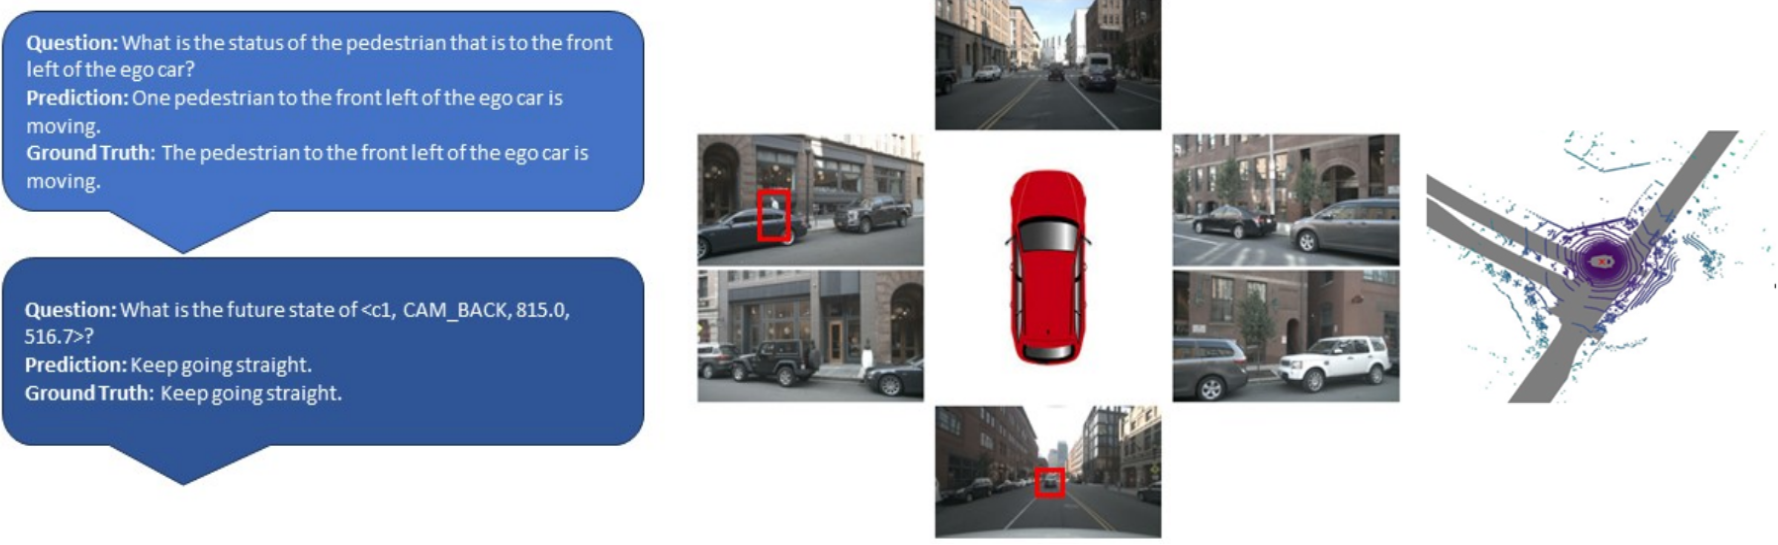
\includegraphics[width=0.9\textwidth]{Figures/Example_QA.png}
    \caption{Example Questions and Visual Inputs for VQA in Driving.}
    \label{fig:example-vqa}
\end{figure}

\paragraph{Contributions.}
\begin{itemize}
    \item We enhance EM-VLM4AD by integrating BEVFusion, allowing rich LiDAR and camera-based spatial encoding.
    \item We achieve the strongest overall balance between fluency (BLEU-4, METEOR) and semantic alignment (ROUGE-L, CIDEr).
    \item We show our model is computationally efficient while improving language output quality over prior baselines.
\end{itemize}


\clearpage


\section{\points{5} Related Work and Background (5 papers per person)}
\paragraph{Related Datasets} 
We build our model and experiments on the \textbf{DriveLM-nuScenes} dataset. DriveLM is a recently proposed benchmark for Graph Visual Question Answering (GVQA) in autonomous driving~\cite{sima2025drivelmdrivinggraphvisual}. It enables multi-stage reasoning over tasks such as perception, prediction, and planning by generating dense, structured QA graphs from real-world driving data. DriveLM-nuScenes in particular is semi-rule-based, combining automated QA generation with human-in-the-loop filtering, and provides over 91 QAs per frame, significantly outpacing earlier driving VQA datasets. 

Table~\ref{tab:related_datasets} provides a comparison between DriveLM and other related datasets in terms of frame count, annotation richness, task coverage, and logic structure. While previous datasets focus on perception or captioning, DriveLM uniquely supports complex, graph-based question answering across the autonomous driving stack.

\begin{table}[H]
\centering
\small
\renewcommand{\arraystretch}{1.25}
\renewcommand\cellgape{}  % Removes top/bottom padding in makecell
\setlength{\tabcolsep}{2pt}  % Shrink column padding here
\begin{tabularx}{\textwidth}{
    >{\raggedright\arraybackslash}m{4.0cm}  % Dataset name column
    >{\raggedright\arraybackslash}m{1.5cm}        % Source dataset
    >{\centering\arraybackslash}m{1.0cm}   % Frames
    >{\centering\arraybackslash}m{1.1cm}   % QA/frame
    >{\centering\arraybackslash}m{1.35cm}   % Perception
    >{\centering\arraybackslash}m{1.35cm}   % Prediction
    >{\centering\arraybackslash}m{1.35cm}   % Planning
    >{\centering\arraybackslash}m{1.0cm}   % Logic
}
\toprule
\textbf{Dataset} & \textbf{Source Dataset} & \textbf{\# Frames} & \textbf{Avg. QA / Frame} & \textbf{Perception} & \textbf{Prediction} & \textbf{Planning} & \textbf{Logic} \\
\midrule
\makecell[tl]{nuScenes-QA\\\cite{qian2024nuscenes}}   & nuScenes & 34,149 & 13.5 & 460k$^{**}$ & \xmark & \xmark & None \\
\makecell[tl]{nuPrompt\\\cite{nuPrompt2023}}           & nuScenes & 34,149 & 1.0  & 35k$^*$     & \xmark & \xmark & None \\
\makecell[tl]{HAD\\\cite{had2023}}                     & HDD      & 25,549 & 1.8  & 25k         & \xmark & 20k     & None \\
\makecell[tl]{BDD-X\\\cite{bai2021bddx}}               & BDD      & 26,228 & 1.1  & 26k         & \xmark & \xmark  & None \\
\makecell[tl]{LingoQA\\\cite{lingoqa2023}}             & LingoQA  & 28,000 & 15.3 & -           & -      & -       & None \\
\makecell[tl]{DRAMA\\\cite{drama2022}}                 & DRAMA    & 17,785 & 5.8  & 85k         & \xmark & 17k     & Chain \\
\makecell[tl]{Rank2Tell\\\cite{rank2tell2023}}         & Rank2Tell& 5,800  & -    & -           & \xmark & -       & Chain \\
\makecell[tl]{DriveLM-CARLA$\dagger$\\\cite{sima2025drivelmdrivinggraphvisual}}     & CARLA    & 64,285 & 24.4 & 697k$^{**}$ & 311k$^{**}$ & 558k$^{**}$ & Graph \\
\makecell[tl]{DriveLM-CARLA$\ddagger$\\\cite{sima2025drivelmdrivinggraphvisual}}    & CARLA    & 5,721  & 24.8 & 63k$^{**}$  & 28k$^{**}$ & 51k$^{**}$  & Graph \\
\makecell[tl]{\textbf{DriveLM-nuScenes}\\\cite{sima2025drivelmdrivinggraphvisual}}   & \textbf{nuScenes} & \textbf{4,871} & \textbf{91.4} & 144k$^*$ & 153k & 146k & \textbf{Graph} \\
\bottomrule
\end{tabularx}
\caption{
Comparison of DriveLM-nuScenes with Existing Vision-Language Datasets. $^*$: semi-rule-based labeling with human annotation. $^{**}$: fully-rule-based annotation. $\dagger$: full dataset. $\ddagger$: keyframe-only dataset.
}
\label{tab:related_datasets}
\end{table}


\paragraph{Unimodal Baselines}
To isolate the impact of visual and spatial inputs, we evaluate a unimodal Q-only baseline, where the model receives only the natural language question as input—without any image or LiDAR data. Specifically, we retain the original input format by concatenating a zero tensor in place of image embeddings, ensuring that the merged multi-modal embedding shape remains unchanged. This setting tests the language model’s ability to infer answers solely from question priors.

We implement this baseline using two encoder-decoder backbones: \textbf{T5-Base} and \textbf{T5-Q-Large}, yielding two variants—Q-only(Base) and Q-only(Q-Large). T5-Base contains 223M parameters, while T5-Q-Large has 757M, enabling a comparison of capacity and efficiency. Interestingly, despite lacking any visual context, both unimodal variants achieve surprisingly competitive performance: BLEU-4 scores of 45.5 and 45.4, and CIDEr scores of 3.09 and 3.10, respectively (Table~\ref{tab:qonly_results}). These results underscore the strong language priors inherent in the dataset.

However, the Q-only models consistently underperform in tasks requiring fine-grained visual grounding and spatial reasoning, highlighting the necessity of multi-modal fusion. Our proposed models, which incorporate both images and LiDAR features, outperform all baselines across ROUGE-L and CIDEr, demonstrating the value of enriched spatial inputs for real-world driving scene understanding.

\begin{table}[H]
\centering
\small
\begin{tabular}{lccccc}
\toprule
\textbf{Methods} & \textbf{BLEU-4} $\uparrow$ & \textbf{METEOR} $\uparrow$ & \textbf{ROUGE-L} $\uparrow$ & \textbf{CIDEr} $\uparrow$ & \textbf{Parameters} $\downarrow$ \\
\midrule
Q-only\textsubscript{Base}   & 45.5 & 34.1 & 70.5 & 3.09 & 223M \\
Q-only\textsubscript{Q-Large}  & 45.4 & 34.0 & 70.1 & 3.10 & 757M \\
\bottomrule
\end{tabular}
\caption{Performance of Unimodal Q-only Baselines using T5-Base and T5-Q-Large on DriveLM-nuScenes VQA Tasks.}
\label{tab:qonly_results}
\end{table}


\FloatBarrier
\paragraph{Prior Work} 
Recent advances in vision-language models (VLMs) have enabled impressive performance across a variety of general-purpose reasoning tasks. However, their application to autonomous driving remains constrained by several limitations: high computational cost, inability to operate in real-time, insufficient support for multi-modal sensor inputs (such as LiDAR and camera), and a lack of structured scene-level reasoning.

Table~\ref{tab:priorwork} summarizes 20 relevant approaches, comparing their core strengths and drawbacks. Existing methods largely fall into two categories: (1) heavy-weight LLMs (e.g., GPT-3.5, BLIP-2) that deliver strong language understanding but are unsuitable for onboard or low-latency deployment; and (2) lightweight or single-view methods that lack spatial context and do not integrate multi-modal data, particularly LiDAR and multi-camera streams. Moreover, most do not provide support for temporally grounded planning or interpretable decision-making.

Our work builds upon the strengths of these models while addressing their limitations through a lightweight architecture that performs multi-view fusion of synchronized camera images and LiDAR point clouds into a BEV (bird's-eye-view) representation. This enables accurate and interpretable graph-based question answering (QA) across perception, prediction, and planning tasks in driving scenarios.

\begin{table}[htbp]
\centering
\small
\begin{tabular}{p{3.2cm} p{5.4cm} p{5.4cm}}
\toprule
\textbf{Paper} & \textbf{Advantage} & \textbf{Disadvantage} \\
\midrule
BLIP-2 \cite{li2023blip2} & Strong zero-shot vision-language reasoning & Heavy model, unsuitable for real-time use \\
GPT-3.5 + CLIP \cite{openai2023gpt4} & Powerful language modeling & High inference latency \\
DriveGPT4 \cite{xu2023drivegpt4} & Generates both answers and low-level control & Uses only single-view images \\
DriveMLM \cite{wang2023drivemlm} & Aligns multimodal inputs including LiDAR and planning state & Very large backbone (LLaMA-7B + ViT-g) \\
LLM-Driver \cite{chen2023driving} & Fuses vectorized representations with LLM & Requires custom grounding \\
VL-T5 \cite{cho2021unifying} & Lightweight text generation from images + text & Single-image only, lacks LiDAR support \\
InstructBLIP \cite{dai2023instructblip} & General-purpose instruction-tuned VLM & Expensive encoder + language model \\
CLIP \cite{radford2021learning} & Powerful vision-text embedding & Not task-optimized, lacks generation \\
ViLT \cite{kim2021vilt} & Transformer-based early fusion V+L & Less accurate on downstream tasks \\
LLaVA \cite{liu2023llava} & Open language-vision model with chat capability & Requires strong image encoder \\
Visual ChatGPT \cite{wu2023visualchatgpt} & Interactive multi-modal answering & Relies on external visual tools \\
MIVC \cite{wu2024mivc} & Attention pooling over visual patches & Still slow due to ViT backbone \\
MiniGPT-4 \cite{zhu2023minigpt4} & Lightweight GPT-4 mimic using BLIP & Brittle on complex tasks \\
VILA \cite{zhao2023vila} & Strong on instruction-following VQA & Limited support for LiDAR or multi-frame \\
EM-VLM4AD \cite{gopalkrishnan2024multi} & Efficient multi-frame T5-based VLM & ViT encoder lacks 3D reasoning \\
BEVFormer \cite{li2022bevformer} & Strong temporal BEV reasoning & Not natively multi-modal \\
BEVFusion \cite{liu2022bevfusion} & Fuses LiDAR + image into BEV & Not designed for VQA \\
TransFusion \cite{bai2022transfusion} & Accurate 3D object detection from LiDAR & No VQA or text interface \\
Point-BERT \cite{yu2022pointbert} & Point cloud self-supervised learning & No cross-modal capabilities \\
DALL-E \cite{ramesh2021dalle} & Visual generation from text & Not interactive or grounded in scene understanding \\
\bottomrule
\end{tabular}
\caption{Analysis of 20 Related Prior Works in Vision-Language and Autonomous Driving.}
\label{tab:priorwork}
\end{table}


\paragraph{Relevant techniques}
Our approach draws inspiration from several core techniques in vision-language and autonomous driving research. First, we leverage \textbf{encoder-decoder transformer architectures}, such as T5, which enable flexible cross-modal reasoning through joint sequence modeling of language and visual embeddings. To support multi-camera spatial understanding, we adopt \textbf{multi-view feature fusion mechanisms}—particularly gated attention pooling for images—to aggregate contextual information from diverse camera viewpoints. For integrating LiDAR, we build on methods like \textbf{BEVFusion}, which aligns point cloud features with image-derived spatial grids for dense scene representation.

To improve training efficiency and parameter scalability, we employ \textbf{Low-Rank Adaptation (LoRA)} modules in the T5 language model. Specifically, we insert lightweight trainable adapters into the attention and MLP sublayers of T5, allowing us to fine-tune only a small subset of parameters while freezing the original backbone. This approach reduces computational cost and mitigates overfitting, enabling more efficient adaptation to domain-specific VQA tasks.

In addition, our QA formulation benefits from \textbf{graph-based reasoning}, where the underlying model is trained to infer structured outputs grounded in object interactions and temporal planning. This builds upon trends in \textbf{multi-modal VQA} and \textbf{driving decision understanding}, extending them toward interpretable and deployable systems. Finally, to benchmark the importance of multi-modal inputs, we incorporate \textbf{zero-embedding masking techniques} in our unimodal baselines (Q-only), following practices in \textbf{ablation-based analysis} to isolate language-only performance.





\clearpage
\section{\points{1} Task Setup and Data}
%Integrate your previous report here
\paragraph{Task Definition.}
We focus on the task of \textbf{graph-based Visual Question Answering (VQA)} in the autonomous driving context, where the goal is to answer natural language questions about driving scenes using both visual and spatial information. Each QA pair is associated with multi-view images, LiDAR point clouds, and object-level annotations. The answers must be interpretable and grounded in scene elements, such as traffic participants, road layout, and dynamic motion.

\paragraph{Dataset.}
We use the \textbf{DriveLM-nuScenes} dataset~\cite{sima2025drivelmdrivinggraphvisual}, which extends the nuScenes dataset with rich visual question answering annotations, having totally 445,279 QA pairs. The QA annotations cover a wide spectrum of driving scenarios and decision-making elements. Each sample includes:
\begin{itemize}
    \item 6 synchronized camera images (front, back, left, right, front-left, front-right)
    \item A LiDAR sweep in the same timestamp
    \item 91.4 QA pairs per frame on average
\end{itemize}

\paragraph{Question Types.}
DriveLM questions are grouped into three major categories: \textbf{Perception}, \textbf{Prediction}, and \textbf{Planning}, with further subcategories illustrated in Figure~\ref{fig:question-distribution} and Figure~\ref{fig:qa-task-distribution}. Perception questions (e.g., “What objects are to the left of the ego vehicle?”) account for 38\% of the data, covering tasks like object identification, traffic sign recognition, and occlusion reasoning. Prediction questions (28\%) involve future motion, object interaction, and attention. Planning questions (24\%) cover safe action reasoning, importance ranking, and high-level decision making.

\paragraph{Templates and Reasoning Complexity.}
QA examples in Table~\ref{tab:qa-templates} highlight the dataset’s diversity and reasoning depth. For instance:
\begin{itemize}
    \item \textbf{Perception:} “What are the objects to the front left of the ego vehicle?”
    \item \textbf{Prediction:} “Will this vehicle likely change motion state based on another?”
    \item \textbf{Planning:} “What is the most probable action for the ego vehicle given the current situation?”
\end{itemize}
Many questions require spatial grounding using camera coordinates (e.g., CAM\_FRONT, 689.2, 527.5) and entail multi-object relational reasoning, temporal logic, or safety evaluation.

\paragraph{Key Objects and Object-Level QA Distribution.}
To further understand what drives the QA composition, we analyze which types of objects are most frequently referenced and how different object categories relate to specific QA types. Figure~\ref{fig:fig9-objects} (left) shows the distribution of key object categories, such as vehicles, pedestrians, and traffic elements (e.g., lights, markings, signs). The middle and right plots break down how question types vary when the subject is a traffic element versus other categories. Notably, traffic-related QAs emphasize spatial grounding and signal semantics (e.g., meaning, position), whereas questions about other objects skew toward motion prediction, planning, and occlusion.

\begin{figure}[H]
    \centering
    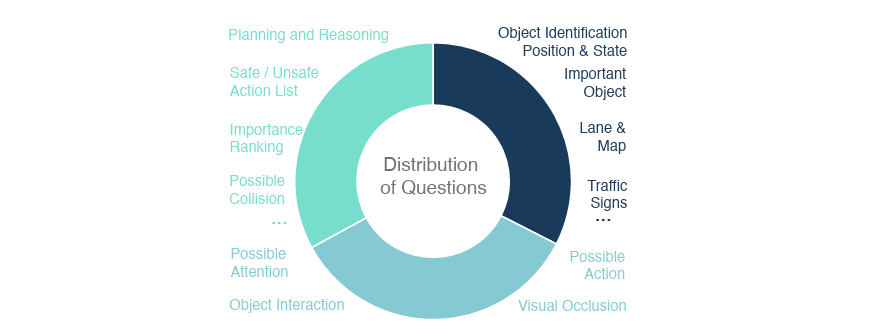
\includegraphics[width=0.8\textwidth]{Figures/DriveLM_Dataset_Fig7.png}
    \caption{High-level Question Types Grouped into Perception, Prediction, and Planning.}
    \label{fig:question-distribution}
\end{figure}

\begin{figure}[H]
    \centering
    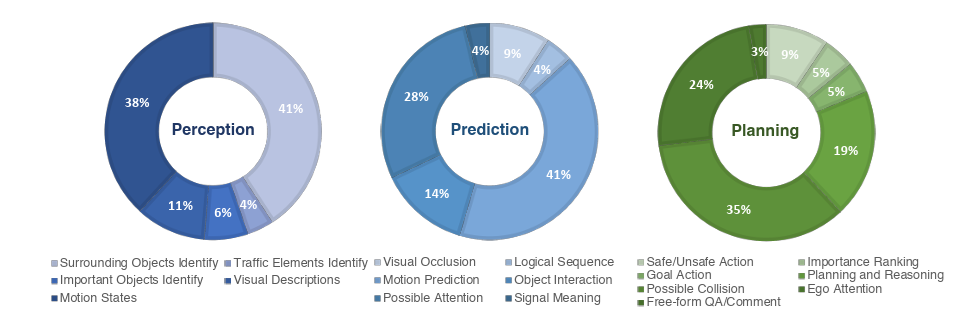
\includegraphics[width=0.9\textwidth]{Figures/DriveLM_Dataset_Fig8.png}
    \caption{Subcategory Breakdown of VQA tasks in DriveLM-nuScenes.}
    \label{fig:qa-task-distribution}
\end{figure}

\begin{table}[H]
    \centering
    \small
    \begin{tabularx}{\textwidth}{>{\bfseries}m{2.4cm} X}
        \toprule
        \textbf{Category} & \textbf{Example Template (Q \& A)} \\
        \midrule
        Perception & Q: What objects are to the front-left of the ego car? \newline A: Two barriers. \\
        Prediction & Q: Will object \texttt{<c1>} change motion due to \texttt{<c2>}? \newline A: No. \\
        Planning & Q: What action should the ego vehicle take in this situation? \newline A: Decelerate without braking. \\
        \bottomrule
    \end{tabularx}
    \caption{Examples of QA Templates at Different Reasoning Levels in DriveLM.}
    \label{tab:qa-templates}
\end{table}

\begin{figure}[H]
    \centering
    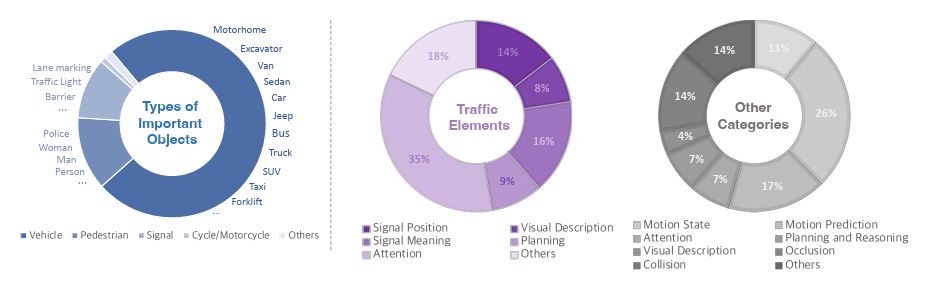
\includegraphics[width=\textwidth]{Figures/DriveLM_Dataset_Fig9.png}
    \caption{(Left) Distribution of Key Object Types Referenced in DriveLM. (Middle) Breakdown of QA Types Associated with Traffic Elements. (Right) Distribution of QA Types for Other Object Categories.}
    \label{fig:fig9-objects}
\end{figure}

\clearpage
\section{\points{1} Baselines}
%Integrate your previous report here
\subsection{Previous Dataset/Baselines}

At the early stage of this project, we adopted the \textbf{NuScenes-QA} dataset~\cite{qian2024nuscenes} as our main VQA benchmark. This dataset extends the original nuScenes perception dataset by adding over \textbf{450,000 question-answer pairs} across more than \textbf{34,000 driving frames}, supporting multi-modal inputs such as RGB images, LiDAR sweeps, and scene-level metadata.

Each QA pair in NuScenes-QA is designed to probe a specific type of reasoning: \textit{Existence}, \textit{Counting}, \textit{Object Recognition}, \textit{Status}, or \textit{Comparison}. Questions are further categorized as either \textit{Zero-Hop} (H0) or \textit{One-Hop} (H1), with H1 questions requiring spatial or relational inference across multiple scene elements.

To evaluate VQA performance on this dataset, we implemented several previously proposed baselines, including both unimodal and multi-modal fusion methods. All models use either the \textbf{Bottom-Up Top-Down (BUTD)} attention module or the \textbf{Modular Co-Attention Network (MCAN)} as the reasoning backend, fed by features extracted from BEVDet (camera), CenterPoint (LiDAR), or both.

\vspace{0.5em}
\textbf{Baseline Summary:}
\begin{itemize}
    \item \textbf{Q-Only:} Only textual question is used; all visual inputs are masked.
    \item \textbf{BEVDet+BUTD / MCAN:} Vision-only baseline using BEV feature maps from multi-camera images.
    \item \textbf{CenterPoint+BUTD / MCAN:} LiDAR-only baseline using 3D bounding boxes and spatial cues.
    \item \textbf{MSMDFusion+BUTD / MCAN:} Multi-sensor fusion combining both BEVDet and CenterPoint.
\end{itemize}

Table~\ref{tab:nuscenes-baselines} reports the Top-1 accuracy across five question categories and two reasoning levels (H0: zero-hop, H1: one-hop) on the NuScenes-QA dataset. Models that incorporate multi-modal fusion (e.g., MSMDFusion+MCAN) consistently outperform unimodal or Q-only baselines, especially in complex reasoning tasks like status and object comparison. The results highlight the importance of both rich visual input and attention-based fusion mechanisms for improving reasoning accuracy in autonomous driving VQA.


\begin{table}[H]
\centering
\scriptsize
\setlength{\tabcolsep}{3pt}
\renewcommand{\arraystretch}{1.2}
\begin{tabular}{l|ccc|ccc|ccc|ccc|ccc|c}
\toprule
\textbf{Models} & \multicolumn{3}{c|}{\textbf{Exist}} & \multicolumn{3}{c|}{\textbf{Count}} & \multicolumn{3}{c|}{\textbf{Object}} & \multicolumn{3}{c|}{\textbf{Status}} & \multicolumn{3}{c|}{\textbf{Comparison}} & \textbf{Acc} \\
 & H0 & H1 & All & H0 & H1 & All & H0 & H1 & All & H0 & H1 & All & H0 & H1 & All & \\
\midrule
Q-Only+BUTD & 81.7 & 78.3 & 79.9 & 18.7 & 18.8 & 18.8 & 63.2 & 40.0 & 43.4 & 57.2 & 49.2 & 52.0 & 81.0 & 64.5 & 66.0 & 54.0 \\
BEVDet+BUTD & 87.2 & 80.6 & 83.7 & 21.7 & 20.0 & 20.9 & 69.4 & 45.2 & 48.8 & 55.0 & 50.5 & 52.0 & 76.1 & 66.8 & 67.6 & 57.0 \\
CenterPoint+BUTD & 87.3 & 80.8 & 83.8 & 21.6 & 20.2 & 20.9 & 67.7 & 43.5 & 47.0 & 67.7 & 51.1 & 54.7 & 76.6 & 65.1 & 66.1 & 56.8 \\
MSMDFusion+BUTD & 89.4 & 81.4 & 85.1 & 25.3 & 21.3 & 23.2 & 73.3 & 48.7 & 52.3 & 67.4 & 55.4 & 59.5 & 81.6 & 67.2 & 68.5 & 59.8 \\
\midrule
Q-Only+MCAN & 81.7 & 78.6 & 80.1 & 18.8 & 18.8 & 18.8 & 64.9 & 40.9 & 44.5 & 56.9 & 45.6 & 49.5 & 80.5 & 65.9 & 67.3 & 54.2 \\
BEVDet+MCAN & 87.2 & 81.7 & 84.2 & 21.8 & 19.2 & 20.4 & 73.0 & 47.4 & 51.2 & 64.1 & 49.9 & 54.7 & 75.1 & 66.7 & 67.4 & 57.9 \\
CenterPoint+MCAN & 87.1 & 82.4 & 84.6 & 21.7 & 20.8 & 21.2 & 69.8 & 50.9 & 53.7 & 64.5 & 56.3 & 59.1 & 75.5 & 66.8 & 67.6 & 59.3 \\
MSMDFusion+MCAN & \textbf{89.0} & \textbf{82.3} & \textbf{85.4} & \textbf{23.4} & \textbf{21.1} & \textbf{22.2} & \textbf{75.3} & \textbf{50.6} & \textbf{54.3} & \textbf{69.0} & \textbf{56.2} & \textbf{60.6} & \textbf{78.8} & \textbf{68.8} & \textbf{69.7} & \textbf{60.4} \\
\bottomrule
\end{tabular}
\caption{Original Baseline Models on NuScenes-QA Showing Top-1 Accuracy across Question Types. H0 = Zero-Hop; H1 = One-Hop.}
\label{tab:nuscenes-baselines}
\end{table}

\subsection{The Problem of the Previous Dataset}
Despite its scale and diversity, a significant portion of the NuScenes-QA dataset suffers from a critical flaw: most QA pairs are misaligned with the corresponding sensor data in the nuScenes dataset. Questions are often paired with incorrect camera images, LiDAR sweeps, or RADAR frames, leading to faulty training signals and unreliable model predictions. Below are representative examples of these misalignments:

\begin{itemize}
    \item \textbf{Example 1:} 
    For example, one QA pair asks: “There is a truck behind the trailer; does it have the same status as the truck to the front-left of the stopped car?” However, the associated images show no truck near the trailer, and the ground-truth answer is “yes”, which is inconsistent with the scene.

\begin{figure}[H]
    \centering
    \begin{subfigure}[t]{0.3\textwidth}
        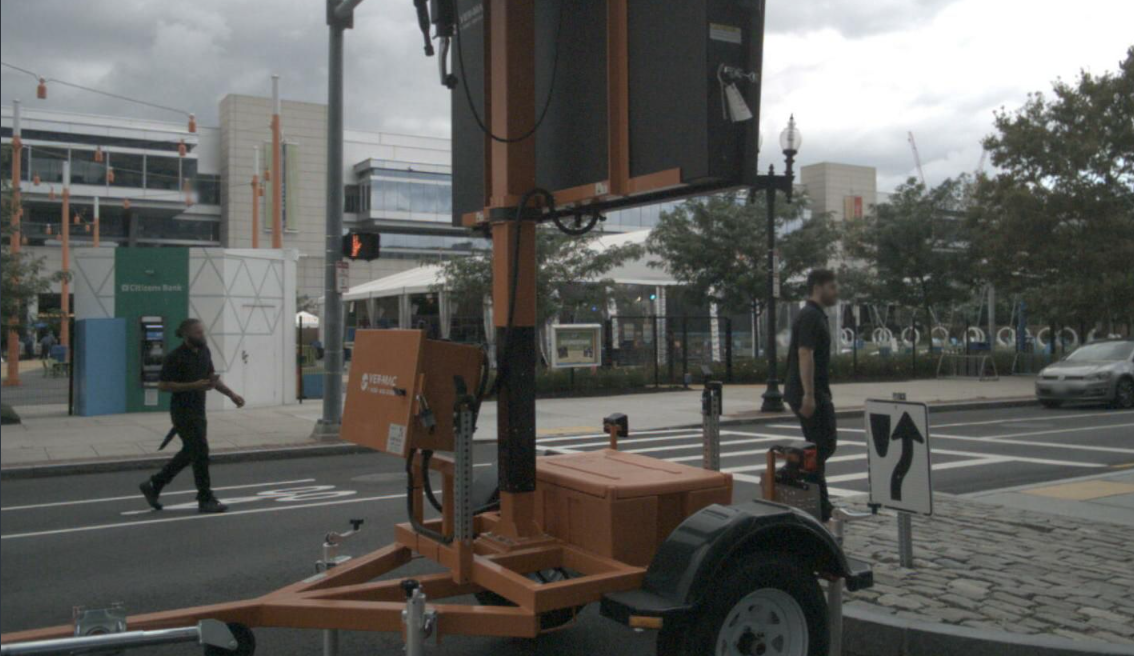
\includegraphics[width=\linewidth]{Figures/exam1_front_left_trailer.png}
        \caption{\small The Trailer is at the Front-Left of the Ego Car.}
    \end{subfigure}
    \hfill
    \begin{subfigure}[t]{0.3\textwidth}
        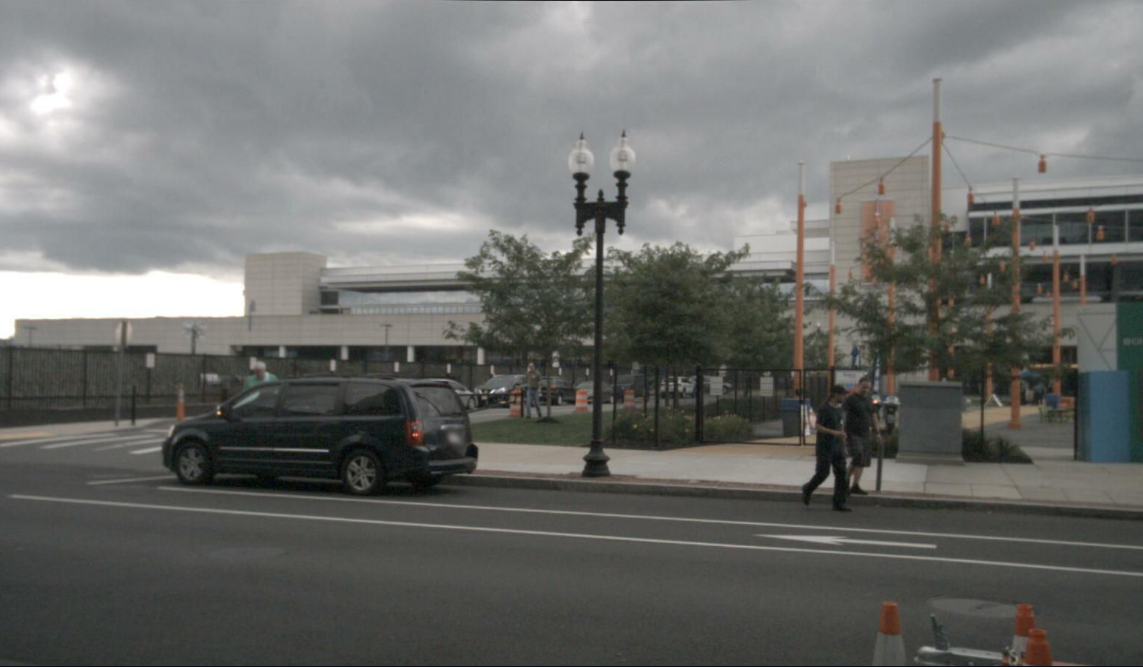
\includegraphics[width=\linewidth]{Figures/exam1_back_left_trailer.png}
        \caption{\small No Truck Exists around the Trailer.}
    \end{subfigure}
    \hfill
    \begin{subfigure}[t]{0.3\textwidth}
        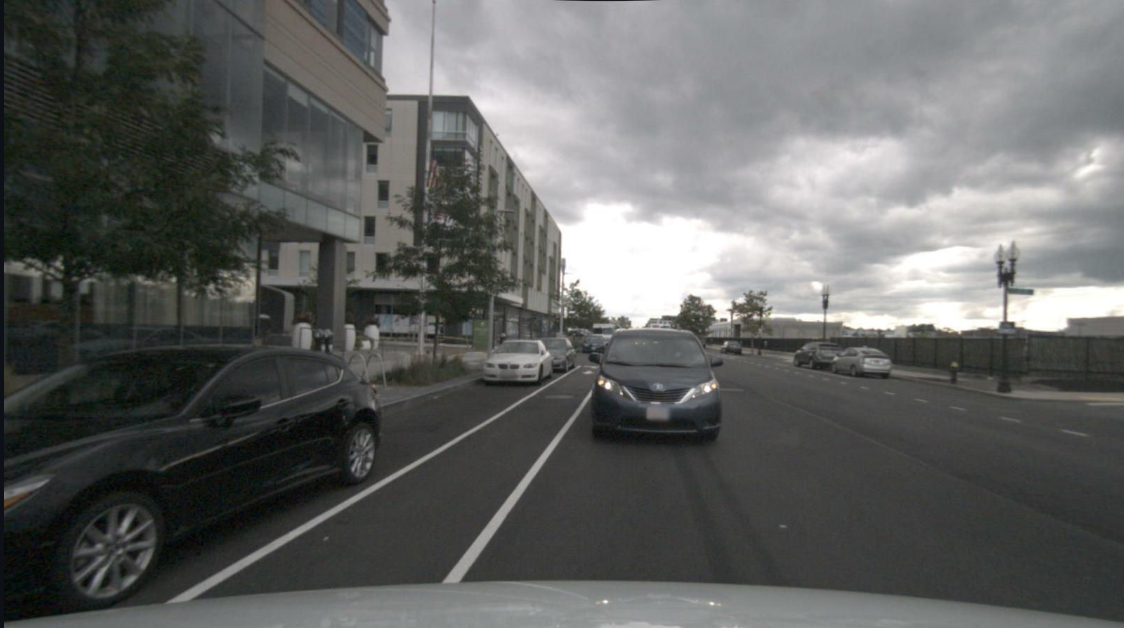
\includegraphics[width=\linewidth]{Figures/exam1_back_trailer.png}
        \caption{\small No Truck Exists to the Back of the Trailer.}
    \end{subfigure}
    \caption{The Front-Left Image (left), Back-Left Image (middle), and the Back Image (right) to the Ego Car.}
    \label{fig:misaligned-examples}
\end{figure}

    \item \textbf{Example 2:} Another example asks: “The truck to the front-left of me is in what status?” with the ground-truth answer “moving”. However, the associated images clearly show no truck present in front of the ego vehicle, further highlighting the misalignment between the QA pair and the corresponding sensor data.
\begin{figure}[H]
    \centering
    \begin{subfigure}[t]{0.3\textwidth}
        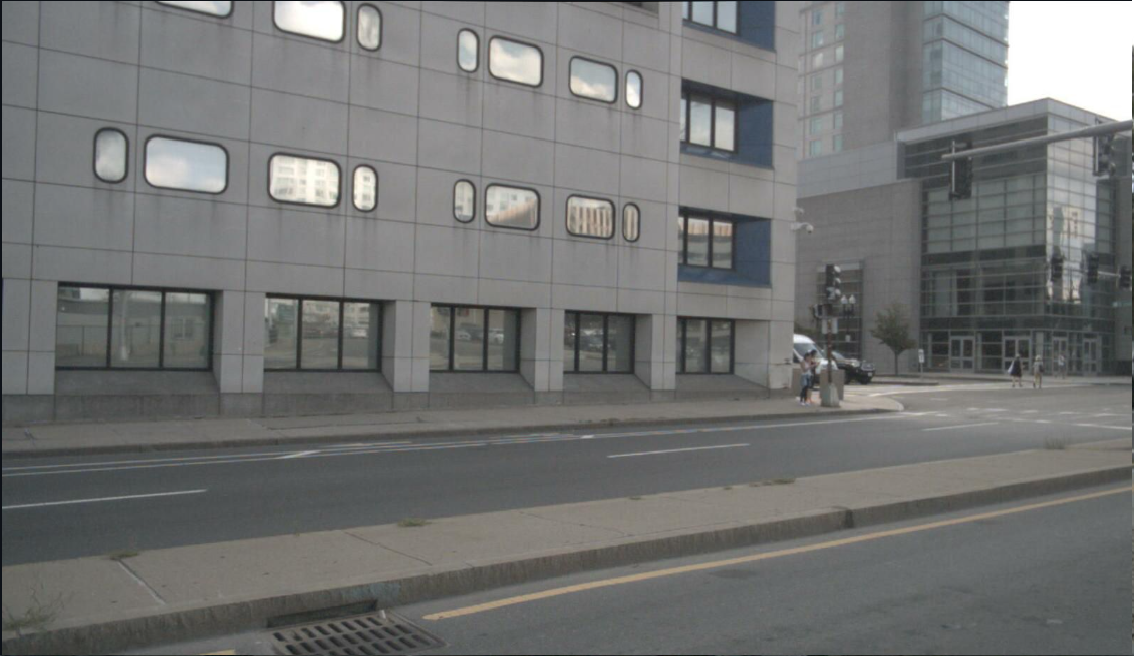
\includegraphics[width=\linewidth]{Figures/exam2_front_left_truck.png}
        \caption{\small No Truck Exists to the Front-Left of the Ego Car.}
    \end{subfigure}
    \hfill
    \begin{subfigure}[t]{0.3\textwidth}
        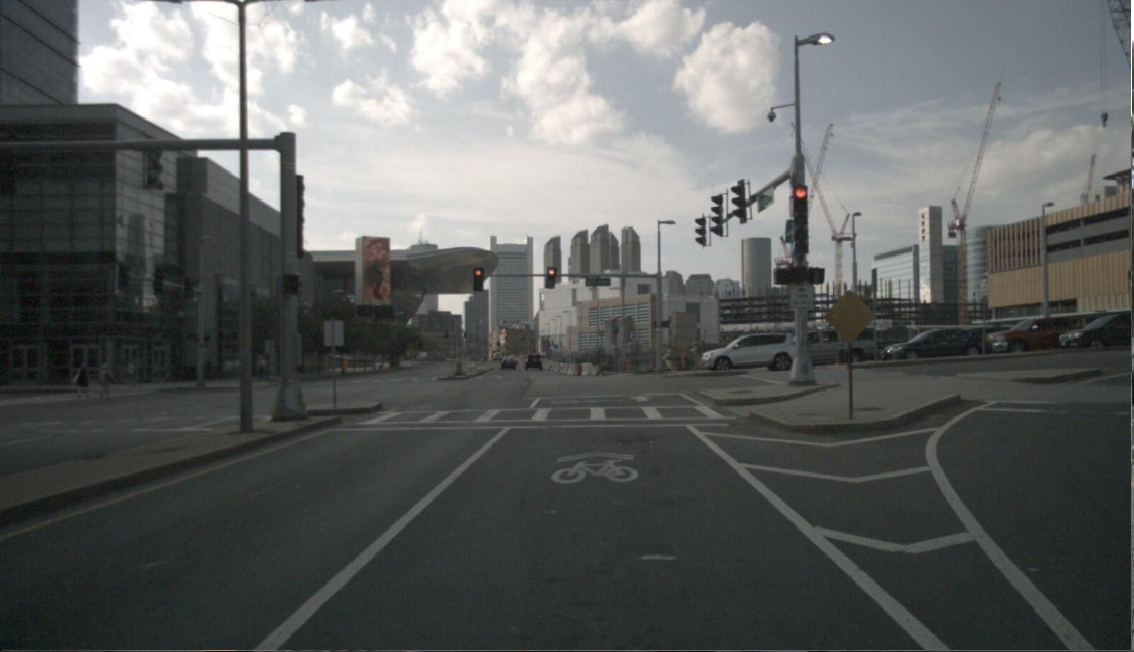
\includegraphics[width=\linewidth]{Figures/exam2_front_truck.png}
        \caption{\small No Truck Exists in the Front of the Ego Car.}
    \end{subfigure}
    \hfill
    \begin{subfigure}[t]{0.3\textwidth}
        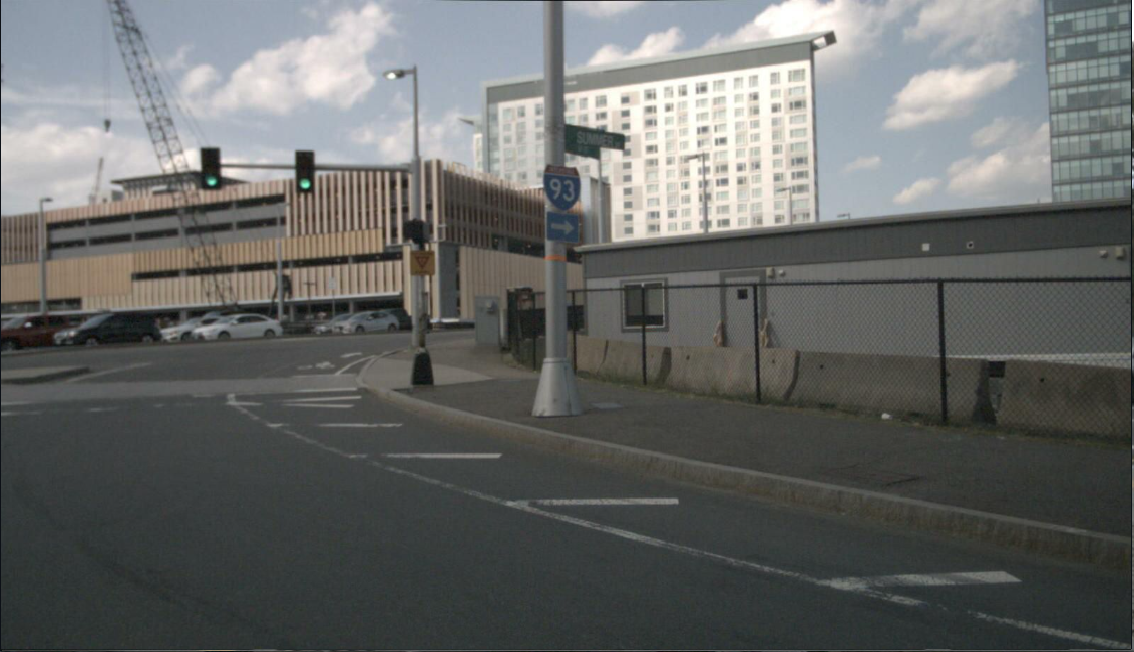
\includegraphics[width=\linewidth]{Figures/exam2_front_right_truck.png}
        \caption{\small No Truck Exists to the Front-Right of the Ego Car.}
    \end{subfigure}
    \caption{The Front-Left Image (left), Front Image (middle), and the Front-Right Image (right) to the Ego Car.}
    \label{fig:misaligned-examples}
\end{figure}    

    \item \textbf{Example 3:} 
    Similarly, another QA pair asks: “What is the status of the pedestrian to the back right of me?” with the ground-truth answer “not standing”. Yet, the sampled camera images show no pedestrian in that region. This misalignment complicates training and undermines supervision quality.
\begin{figure}[H]
    \centering
    \begin{subfigure}[t]{0.3\textwidth}
        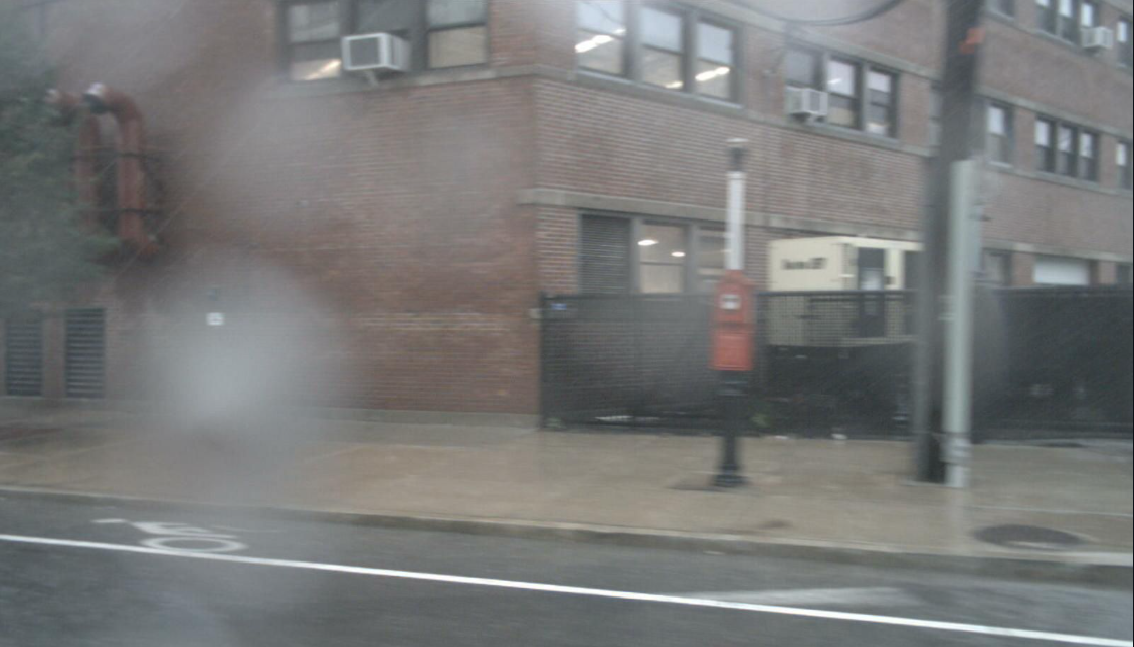
\includegraphics[width=\linewidth]{Figures/exam3_back_left_ped.png}
        \caption{\small No Pedestrian Exists to the Back-Left of the Ego Car.}
    \end{subfigure}
    \hfill
    \begin{subfigure}[t]{0.3\textwidth}
        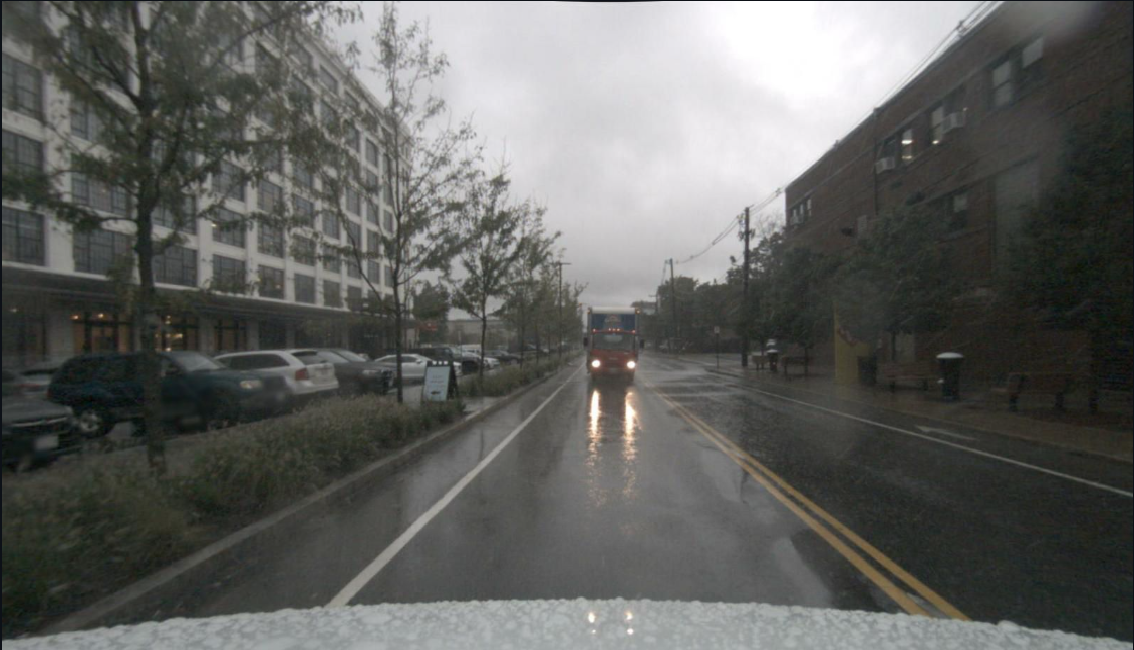
\includegraphics[width=\linewidth]{Figures/exam3_back_ped.png}
        \caption{\small No Pedestrian Exists in the Back of the Ego Car.}
    \end{subfigure}
    \hfill
    \begin{subfigure}[t]{0.3\textwidth}
        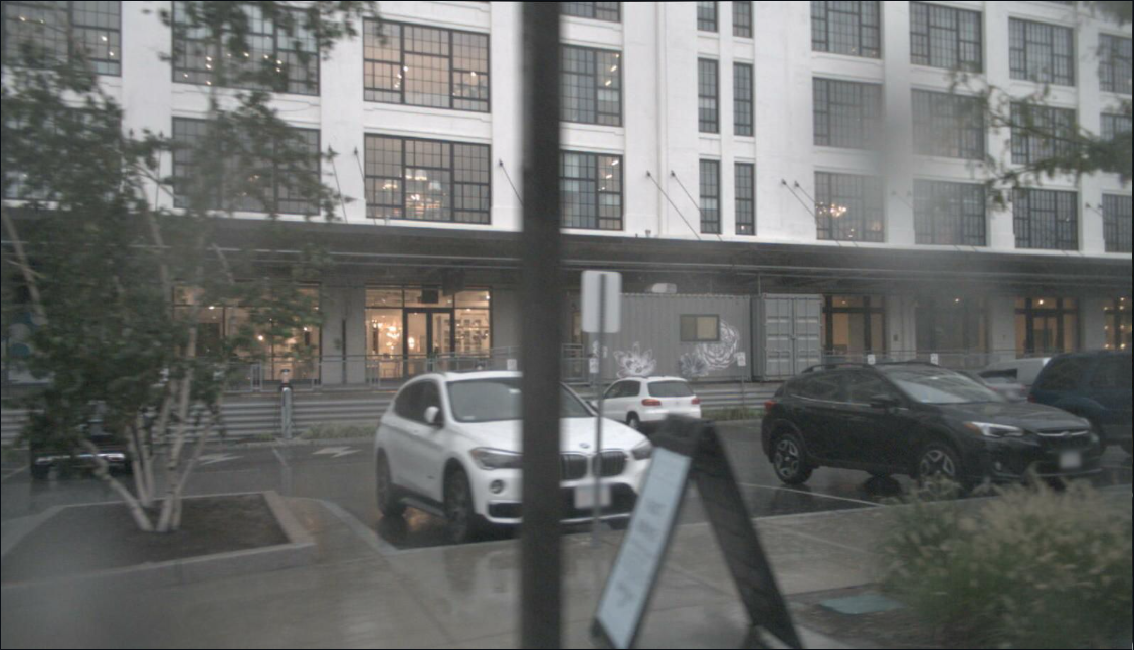
\includegraphics[width=\linewidth]{Figures/exam3_back_right_ped.png}
        \caption{\small No Pedestrian Exists to the Back-Right of the Ego Car.}
    \end{subfigure}
    \caption{The Back-Left Image (left), Back Image (middle), and the Back-Right Image (right) to the Ego Car.}
    \label{fig:misaligned-examples}
\end{figure}   

\end{itemize}


\subsection{New Dataset/Baselines}
Due to the critical misalignment issues between QA pairs and sensor data in the NuScenes-QA dataset, we adopt a new dataset: \textbf{DriveLM-nuScenes}~\cite{gopalkrishnan2024multi}. Unlike NuScenes-QA, DriveLM provides accurate matching between each QA pair and the corresponding sensor data—including multi-view images, LiDAR, and object annotations—ensuring reliable visual grounding and interpretable outputs.

DriveLM-nuScenes contains 4,871 keyframes and 91.4 QA pairs per frame on average. Each QA is associated with a full set of six camera images and a synchronized LiDAR scan, enabling the model to reason over complete 360° driving scenes. Questions span a wide range of tasks: perception, prediction, and planning, covering object status, spatial reasoning, occlusions, and safe action planning.

We benchmark the following baselines on the new dataset with detailed metrics in Table~\ref{tab:merged-drive-performance}:

\begin{itemize}
    \item \textbf{Q-only (T5-Base / T5-Q-Large):} These models receive only the textual question as input. Visual embeddings are replaced with zero tensors, maintaining the same embedding size. T5-Base has 223M parameters, while T5-Q-Large has 757M, allowing comparison of language model capacity.
    
    \item \textbf{EM-VLM4AD (T5-Base / T5-Q-Large):} These multimodal models integrate image features with T5-based language models. The “Base” variant uses a lightweight encoder, while “Q-Large” adopts a larger T5 model with stronger linguistic capacity.
    
    \item \textbf{DriveLM-Agent:} A vision-language model based on BLIP-2 and Flan-T5-XL, which takes a front-view RGB image and a text prompt as input. The model performs trajectory-aware reasoning by decoding future waypoints as token sequences, using a specially designed inverse mapping to embed real-world trajectory coordinates into the language model’s token space.

\end{itemize}

\vspace{1mm}

\begin{table}[H]
    \centering
    \small
    \begin{tabular}{lccccr}
        \toprule
        \textbf{Model} & \textbf{BLEU-4} $\uparrow$ & \textbf{METEOR} $\uparrow$ & \textbf{ROUGE-L} $\uparrow$ & \textbf{CIDEr} $\uparrow$ & \textbf{Params} $\downarrow$ \\
        \midrule
        Q-only\textsubscript{Base}       & 45.50  & 34.10  & 70.50  & 3.09 & 223M \\
        Q-only\textsubscript{Q-Large}      & 45.40  & 34.03  & 70.10  & 3.10 & 757M \\
        EM-VLM4AD$_\text{Base}$   & 45.36 & 34.49 & \textbf{71.98} & \textbf{3.20}  & 235M \\
        EM-VLM4AD$_\text{Q-Large}$ & 40.11 & 34.34 & 70.72 & 3.10  & 769M \\
        DriveLM-Agent~\cite{gopalkrishnan2024multi} & \textbf{53.09} & \textbf{36.19} & 66.79 & 2.79 & 3.96B \\
        \bottomrule
    \end{tabular}
    \caption{Comparison of Baseline Models on DriveLM-nuScenes. Q-only models use text only; others incorporate image features.}
    \label{tab:merged-drive-performance}
\end{table}



\clearpage
\section{\points{3} Proposed Model ($>$1 page)}
%This is not a copy and page from R2, it should be updated to reflect the final proposed model. Explain if there are multiple versions (e.g. your model has possible extensions, different amounts of exemplars, etc).  Include an easy to read model diagram here.
Our proposed model fuses image and LiDAR modalities using BEVFusion, generating geometrically grounded visual features that capture both semantic appearance and spatial geometry. As shown in Figure~\ref{fig:drivelm-arch}, we use a dual-branch encoder: a camera encoder extracts features from multi-view RGB images, while a LiDAR encoder encodes point clouds. These are aligned in a shared Bird's Eye View (BEV) space and fused using spatial-aware convolution.

The resulting BEV features are flattened and concatenated with a language embedding sequence (corresponding to the input question tokens). This joint representation is then passed to a pre-trained T5 model (either Base or Q-Large), which acts as a multimodal decoder. We fine-tune this architecture end-to-end to generate natural language answers for graph-based QA tasks.

This unified pipeline enables spatially grounded reasoning across perception, prediction, and planning tasks, benefiting from the complementary strengths of image appearance and LiDAR depth information.

\begin{figure}[H]
    \centering
    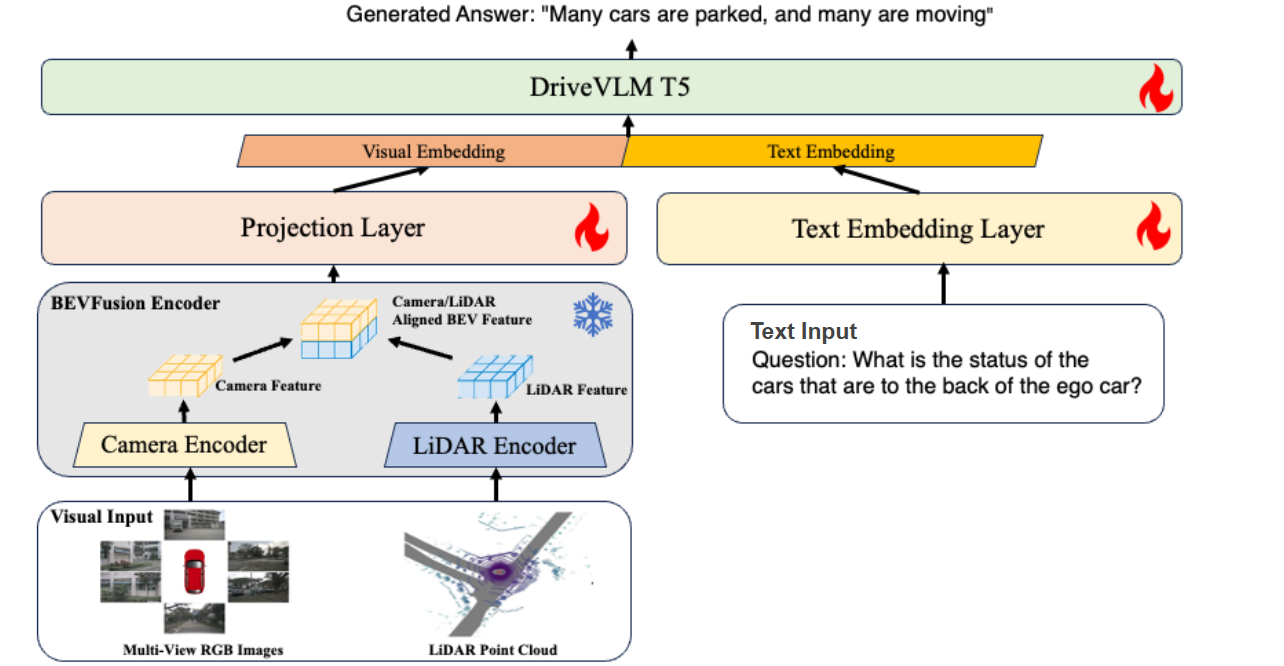
\includegraphics[width=0.95\linewidth]{Figures/proposed_model_arch.png}
    \caption{Proposed Model Architecture}
    \label{fig:drivelm-arch}
\end{figure}

\subsection{Loss functions}

%Our model is based on the LLM model T5\cite{Raffel2019ExploringTL}. 
In the Visual Question Answering (VQA) task, the model output is a sequence of token IDs representing the predicted text. During training, we tokenize the ground-truth answers into token ID sequences as well. We then apply the cross-entropy loss between the predicted token distribution and the ground-truth token IDs. The loss function is formulated as:

%$\mathcal{L}{\text{CE}} = -\frac{1}{N} \sum{i=1}^{N} \sum_{t=1}^{T_i} \log p_{\theta}(y_t^{(i)} \mid y_{<t}^{(i)}, x^{(i)})$

\[
\mathcal{L}_{\text{CE}} = -\frac{1}{N} \sum_{i=1}^{N} \sum_{t=1}^{T_i} \log p_{\theta}(y_t^{(i)} \mid y_{<t}^{(i)}, x^{(i)})
\]

where N is the batch size, $T_i$ is the length of the i-th ground truth token sequence, $y_t^{(i)}$ is the ground truth token at time step t, $y_{<t}^{(i)}$ are the previous ground truth tokens, $x^{(i)}$ is the input (e.g., features and question), and $p_{\theta}$ is the model’s predicted probability distribution parameterized by $\theta$.


\subsection{Changes to training data}

%The DriveLM dataset we used is originally from the Nuscenes Dataset\cite{Caesar2019nuScenesAM}, which contains multi-modality raw data including images and LiDAR data we need. The baseline model EM-VLM4AD only use the images as input. To extract image features, the model adopt the patch embedding strategy from ViT~\cite{Dosovitskiy2020AnII}. Given an input RGB image $I \in \mathbb{R}^{3 \times H \times W}$, we divide it into patches, flatten them, and apply a linear projection followed by positional encoding. This results in a sequence of latent image embeddings:

%$$
%V_i \in \mathbb{R}^{S_I \times H_I}
%$$

%where $S_I$ is the number of image patches (i.e., sequence length), and $H_I$ is the hidden dimension of each patch embedding. We use a ViT-B/32 model pretrained on ImageNet~\cite{Deng2009ImageNetAL} to generate these embeddings.

%Our model uses BEVFusion~\cite{Liu2022BEVFusionMM} as the feature fusion module. BEVFusion unifies multi-modal features in the shared bird’s-eye view (BEV) representation space, which nicely preserves both geometric and semantic information. Specifically, the BEVFusion model adopt a Swin-T~\cite{Liu2021SwinTH} model as the image encoder and a VoxelNet~\cite{Zhou2017VoxelNetEL} as the LiDAR encoder. After collecting the image feature and LiDAR feature, the model will

The DriveLM dataset we used is originally derived from the nuScenes dataset~\cite{Caesar2019nuScenesAM}, which contains multi-modal raw data including 6-camera RGB images and LiDAR sweeps for each key sample. In the original form of DriveLM-nuScenes dataset, each QA pair is annotated with the question, answer, and six corresponding camera images from the nuScenes scene. However, to enable geometrically grounded reasoning and leverage complementary spatial information, we augment the original QA pairs by incorporating aligned LiDAR sweeps for each sample. This extension allows our model to benefit from both visual appearance cues (from images) and accurate depth geometry (from LiDAR), which is critical for spatial reasoning in driving scenarios.

For the baseline EM-VLM4AD model, only the images are used as input. To extract visual features, it adopts the patch embedding strategy from ViT~\cite{Dosovitskiy2020AnII}. Given an input RGB image $I \in \mathbb{R}^{3 \times H \times W}$, the image is divided into patches, flattened, and passed through a linear projection followed by positional encoding. This results in a sequence of latent image embeddings:

\[
V_i \in \mathbb{R}^{S_I \times H_I}
\]

where $S_I$ is the number of image patches (i.e., sequence length), and $H_I$ is the hidden dimension of each patch embedding. We use a ViT-B/32 model pretrained on ImageNet~\cite{Deng2009ImageNetAL} to generate these embeddings.

Our model uses BEVFusion~\cite{Liu2022BEVFusionMM} as the core feature fusion module. BEVFusion unifies multi-modal features into a shared bird’s-eye view (BEV) representation, preserving both geometric precision and semantic richness. Specifically, we employ a Swin-T~\cite{Liu2021SwinTH} network as the image encoder and a VoxelNet~\cite{Zhou2017VoxelNetEL} as the LiDAR encoder. These encoders produce camera and LiDAR features that are projected into the BEV space. The resulting BEV-aligned features from both modalities are fused, serving as input to the downstream QA model.

\subsection{Training Setup}
We train two versions of our model based on different backbone sizes: one using T5-Base and the other using T5-Large with LoRA fine-tuning (T5-Q-Large). All training is performed on a single NVIDIA RTX A6000 GPU.

The T5-Base model is trained for eight epochs, taking approximately 20 hours to complete, while the T5-Q-Large model requires about two days to finish training for eight epochs. We note that, due to the lightweight nature of our method, the T5-Base version can be easily accommodated within a single T4 GPU instance, allowing for free evaluation on platforms such as Google Colab.

For all models, we use a learning rate of $5\times10^{-4}$, a weight decay of $0.05$, an exponential learning rate scheduler, and a batch size of $4$.





\subsection{Hyperparameters and their effects}


We study the impact of several key hyperparameters on the model’s final performance, measured by BLEU-4, METEOR, ROUGE-L, and CIDEr. Below, we detail the experimental settings and findings for three important hyperparameters as the following:

\paragraph{1. Learning Rate.}
We analyze the effect of different learning rates ($1\text{e}{-5}$, $1\text{e}{-4}$, and $5\text{e}{-4}$) on the final performance of the T5-Base model with BEVFusion features under both non-pretrained and pretrained settings.

Without pretraining (Table~\ref{tab:lr_effectwopretrain}), a small learning rate of $1\text{e}{-5}$ results in poor performance across all metrics, suggesting underfitting and slow convergence. Increasing the learning rate to $1\text{e}{-4}$ yields significant improvements in BLEU-4, METEOR, ROUGE-L, and CIDEr. A further increase to $5\text{e}{-4}$ provides marginal gains in BLEU-4 and ROUGE-L, but slightly reduces METEOR, indicating that while the model benefits from faster learning dynamics, overly aggressive updates may hinder fine-grained alignment. This suggests that $5\text{e}{-4}$ is effective in promoting expressive outputs, but $1\text{e}{-4}$ provides a slightly more balanced optimization.
\begin{table}[H]
    \centering
    \small
    \begin{tabular}{lcccc}
        \toprule
        \textbf{LR} & \textbf{BLEU-4} & \textbf{METEOR} & \textbf{ROUGE-L} & \textbf{CIDEr} \\
        \midrule
        $1e{-5}$   & 40.54 & 32.05 & 68.69 & 2.75 \\
        $1e{-4}$   & 50.04 & \textbf{36.79} & 73.59 & \textbf{3.32} \\
        $5e{-4}$   & \textbf{50.57} & 36.52 & \textbf{73.74} & 3.31 \\
        \bottomrule
    \end{tabular}
    \caption{Effect of Learning Rate on Final Metrics without Pretraining Stage 8 epochs.}
    \label{tab:lr_effectwopretrain}
\end{table}

With pretraining (Table~\ref{tab:lr_effectwpretrain}), the learning rate has a more nuanced impact. The lowest learning rate ($1\text{e}{-5}$) achieves the best BLEU-4 (49.66), indicating accurate token-level alignment with ground-truth captions. However, the highest learning rate ($5\text{e}{-4}$) leads to the best METEOR (36.82), ROUGE-L (74.56), and CIDEr (3.36) scores, highlighting that a moderately larger learning rate helps the model generate more fluent, diverse, and semantically rich descriptions. This contrast suggests that pretrained models are more stable and can leverage higher learning rates to improve generalization, while smaller rates may restrict learning to exact matching.

\begin{table}[H]
	\centering
	\small
	\begin{tabular}{lcccc}
		\toprule
		\textbf{LR} & \textbf{BLEU-4} & \textbf{METEOR} & \textbf{ROUGE-L} & \textbf{CIDEr} \\
		\midrule
		$1e{-5}$   & \textbf{49.66} & 36.03 & 73.23 & 3.31 \\
		$1e{-4}$   & 48.86 & 35.99 & 74.13 & 3.33 \\
		$5e{-4}$   & 48.95 & \textbf{36.82} & \textbf{74.56} & \textbf{3.36} \\
		\bottomrule
	\end{tabular}
	\caption{Effect of Learning Rate on Final Metrics with Pretraining Stage 8 epochs.}
	\label{tab:lr_effectwpretrain}
\end{table}

In summary, without pretraining, a moderate learning rate ($1\text{e}{-4}$ or $5\text{e}{-4}$) is necessary for effective convergence. With pretraining, higher learning rates like $5\text{e}{-4}$ allow the model to better exploit the initialization and produce richer captions, though at the slight expense of exact match accuracy.


\paragraph{2. Switch Between T5-Base/T5-Q-Large LLM models.}

We explore the effect of switching between T5-Base and T5-Q-Large as the backbone language model for our method. As shown in Table~\ref{tab:llm-effect}, we train two models with different LLM sizes: T5-Base and T5-Q-Large.

Specifically, we use two different pre-trained versions of the T5 language model: \textbf{T5-Base}, which contains approximately 223 million parameters, and an \textbf{8-bit quantized version of T5-Large}, which has around 750 million parameters. Using these pre-trained LMs, we perform fine-tuning to adapt the language model to the concatenated BEV features and text embeddings.

For the T5-Base model, we find that fine-tuning the entire model leads to the best performance. In contrast, for the quantized T5-Large model, we employ LoRA-Fine-Tuning-Aware Quantization~\cite{li2023loftq}, which minimizes quantization error by carefully initializing the LoRA weights during training.

Table~\ref{tab:llm-effect} compares the performance of T5-Base and T5-Q-Large when fine-tuned with BEVFusion features. While T5-Q-Large achieves a slightly higher BLEU-4 score (\textbf{49.54}), indicating stronger surface-level n-gram overlap with ground truth answers, T5-Base achieves the best scores across METEOR (\textbf{36.82}), ROUGE-L (\textbf{74.56}), and CIDEr (\textbf{3.36}). These metrics suggest that T5-Base generates responses with better semantic coverage, longer-span fluency, and alignment with human-like answers. Despite its smaller size, T5-Base proves more effective in capturing essential information for driving-related QA, possibly due to more stable fine-tuning dynamics or better adaptation to structured visual input.


\begin{table}[h]
    \centering
    \small
    \begin{tabular}{lcccc}
        \toprule
        \textbf{LLM Model} & \textbf{BLEU-4} & \textbf{METEOR} & \textbf{ROUGE-L} & \textbf{CIDEr} \\
        \midrule
T5-Base             & 48.95 & \textbf{36.82} & \textbf{74.56} & \textbf{3.36} \\
T5-Q-Large & \textbf{49.54} & 36.73          & 73.51          & 3.29\\
        \bottomrule
    \end{tabular}
    \caption{Effect of LLM Models on Final Metrics.}
    \label{tab:llm-effect}
\end{table}



\paragraph{3. BEV Feature Projection Layer Complexity.}

We also investigate how the complexity of projection layers affects the model performance. In our original BEVFusion design, the projection layer consists of only a single linear layer that aligns the BEVFusion features with the text embeddings. We are interested in exploring whether using more complicated projection layers (multiple projection layers with more parameters) can lead to better performance comparing with the original one.


\begin{table}[h]
    \centering
    \small
    \begin{tabular}{lccccc}
        \toprule
        \textbf{\# of the projection layers} & \textbf{\# of parameters} & \textbf{BLEU-4} & \textbf{METEOR} & \textbf{ROUGE-L} & \textbf{CIDEr} \\
        \midrule
one layer
& 33,177,600 & \textbf{48.95} & \textbf{36.82} & \textbf{74.56} & \textbf{3.36} \\
two layers & 33,964,032 & 48.62 & 35.71 & 73.44& 3.27\\
        \bottomrule
    \end{tabular}
    %\caption{Effect of \# of Projection layers}
    \caption{Effect of of Projection Layers Complexity}
    \label{tab:proj-effect}
\end{table}


As shown in the Table~\ref{tab:proj-effect}, we find that increasing the complexity of the projection layers, by adding an additional linear layer, slightly increases the number of parameters but does not lead to performance improvement. In fact, the model with a single projection layer achieves better or comparable results across most metrics (BLEU-4, ROUGE-L, and CIDEr). This means a simple single-layer projection is sufficient for aligning BEV features with text embeddings, and adding more layers introduces unnecessary complexity with the risk of overfitting.



\clearpage
%\begin{table}[t]
%\centering
%\begin{tabular}{@{}lrr@{}}
%\toprule
                            %& \multicolumn{2}{c}{Dev} \\
%Methods                     & Accuracy $\uparrow$ & $L_2$ Error $\downarrow$  \\
%\midrule
%Q-only \cite{} & & \\
% Unimodal 2 \cite{} & & \\
% Unimodal 3 \cite{} & & \\
%\midrule
%Simple Multimodal 1 \cite{} & & \\
%Simple Multimodal 2 \cite{} & & \\
%Simple Multimodal 3 \cite{} & & \\
%\midrule
%Previous Approach 1 \cite{} & & \\
%Previous Approach 2 \cite{} & & \\
%Previous Approach 3 \cite{} & & \\
%\midrule
%Proposed Method (v1)            & & \\
%Proposed Method (v2)            & & \\
%Proposed Method (final)            & & \\
%\bottomrule
%\end{tabular}
%\end{table}


\section{\points{1} Results (1 page)}
% Replace columns with the correct metrics for your task (extrinsic). Include multiple versions of your final model.  You do not need to run on the test set but are encouraged to try if you have nice results on Dev.

We evaluate our models on the DriveLM-nuScenes benchmark using four standard language generation metrics: \textbf{BLEU-4}, \textbf{METEOR}, \textbf{ROUGE-L}, and \textbf{CIDEr}, as well as reporting the model \textbf{parameter size}.

\begin{itemize}
    \item \textbf{BLEU-4} measures the precision of 4-gram overlaps between generated and reference text, rewarding exact matches over short sequences.
    \item \textbf{METEOR} considers both precision and recall, aligning words semantically, and penalizing fragmentation, making it more sensitive to synonyms and paraphrasing.
    \item \textbf{ROUGE-L} computes the longest common subsequence between the prediction and the ground truth, emphasizing overall structure matching.
    \item \textbf{CIDEr} evaluates consensus by weighting n-grams based on their importance across a set of references, and is particularly effective in measuring relevance for descriptive tasks.
\end{itemize}

As shown in Table~\ref{tab:results}, our models (\textbf{Ours\textsubscript{Base}} and \textbf{Ours\textsubscript{Q-Large}}) outperform prior baselines across most evaluation metrics. Notably, \textbf{Ours\textsubscript{Base}} achieves the highest scores in METEOR (\textbf{36.8}), ROUGE-L (\textbf{74.6}), and CIDEr (\textbf{3.36}), demonstrating strong capabilities in generating semantically rich and consensus-aligned answers. In addition, \textbf{Ours\textsubscript{Q-Large}} achieves the second-best BLEU-4 score (\textbf{49.5}), just behind DriveLM-Agent, while using significantly fewer parameters. These results highlight the effectiveness of our approach in balancing precision, fluency, and efficiency.

While BLEU-4 scores remain competitive, the significant improvements in CIDEr and ROUGE-L suggest that our generated outputs are richer and better aligned with human expectations. 

Furthermore, despite using significantly fewer parameters than large baseline models such as DriveLM-Agent, our models maintain strong performance across all metrics, highlighting the efficiency and scalability of our approach.

\begin{table}[H]
\centering
\resizebox{\linewidth}{!}{
\begin{tabular}{@{}lccccc@{}}
\toprule
Methods                     & BLEU-4 $\uparrow$ & METEOR $\uparrow$ & ROUGE-L $\uparrow$ & CIDEr $\uparrow$ & Parameters $\downarrow$\\
\midrule
Q-only\textsubscript{Base} & 45.5 & 34.1 & 70.5 & 3.09 & 223M \\
Q-only\textsubscript{Q-Large}  & 45.4 & 34.0 & 70.1 & 3.10 & 757M \\
\midrule
DriveLM-Agent \cite{sima2025drivelmdrivinggraphvisual} & \textbf{53.1} & 36.2 & 66.8 & 2.79 & 3.96B \\
\midrule
EM-VLM4AD\textsubscript{Base} \cite{gopalkrishnan2024multi} & 45.4 & 34.5 & 72.0 & 3.20 & 235M\\
EM-VLM4AD\textsubscript{Q-Large} \cite{gopalkrishnan2024multi} & 40.1 & 34.3 & 70.7 & 3.10 & 769M\\
\midrule
Ours\textsubscript{Base}
& 49.0 & \textbf{36.8} & \textbf{74.6} & \textbf{3.36} & 288M\\
Ours\textsubscript{Q-Large} & 49.5 & 36.7 & 73.5 & 3.29 & 822M\\
\bottomrule
\end{tabular}
}
\caption{Comparison of Our Methods with Baseline Models on DriveLM-nuScenes.}
\label{tab:results}
\end{table}

\clearpage
\section{\points{3} Analysis (2 pages)}
%This section should include plots.  For example, how key metrics vary with a specific hyperparameter, task complexity, etc.

\subsection{Intrinsic Metrics}
Intrinsic metrics are not directly tied to the task output but rather reflect the essential skills the model should possess. They may overlap with auxiliary losses but serve as independent indicators of model quality.

Our work focuses on a visual question answering (VQA) task under an autonomous driving scenario. Based on previous research on autonomous driving VQA tasks, such as nuScenes-QA~\cite{qian2024nuscenes}, we observed that higher detection and localization quality directly correlate with improved VQA performance. Therefore, we adopt two widely used metrics in autonomous driving to measure the quality of the extracted features, as detailed below.

\paragraph{Intrinsic Metric 1}

Since our work is based on the nuScenes dataset \cite{Caesar2019nuScenesAM}, we adopt the mean Average Precision (mAP) as evaluation metrics. The mAP is defined as the mean of the average precision over ten classes, evaluated under distance thresholds of 0.5m, 1m, 2m, and 4m:

\begin{equation}
\text{mAP} = \frac{1}{C} \sum_{c=1}^{C} \text{AP}_c
\end{equation}

Where C denotes the total number of classes (10 in the case of nuScenes), and $\text{AP}_c$ represents the Average Precision for class c, computed over multiple distance thresholds (0.5m, 1m, 2m, 4m). The final mAP is obtained by averaging across all classes.

\paragraph{Intrinsic Metric 2}

The nuScenes Detection Score (NDS) is a weighted combination of mAP and five True Positive error metrics: mean Average Translation Error (mATE), mean Average Scale Error (mASE), mean Average Orientation Error (mAOE), mean Average Velocity Error (mAVE), and mean Average 
Attribute Error (mAAE):

\begin{equation}
\text{NDS} = \frac{1}{10} \left[5 \cdot \text{mAP} + \sum_{m \in \mathcal{M}} (1 - \min(1, m)) \cdot 100 \right]
\end{equation}

Where $\mathcal{M} = \{\text{mATE}, \text{mASE}, \text{mAOE}, \text{mAVE}, \text{mAAE} \}$ represents the five True Positive error metrics.

Each metric is better when smaller, so the score component is computed as $(1 - \min(1, m))$.
The final NDS is a weighted combination of mAP and the five error metrics, normalized to a score between 0 and 100.

The results are summarized in Table~\ref{tab:intrinsic}. BEVFusion achieves the best performance in both mAP and NDS among all compared methods, which aligns with its superior results in the final VQA tasks.


\begin{table}[H]
\centering
\begin{tabular}{@{}lrr@{}}
\toprule
Methods & MAP & NDS  \\
\midrule
%Q-only (Unimodal) \cite{}       & - & - \\
CenterPoint (Simple model)   & 0.3754 & 0.4408 \\
PETR (Simple model)         & 0.3830 & 0.3912 \\
BEVFusion (Multimodal)            & 0.5209 & 0.4657 \\
\bottomrule
\end{tabular}
\caption{A Complete Table of Intrinsic Metrics}
\label{tab:intrinsic}
\end{table}







% \begin{table}[t]
% \centering
% \begin{tabular}{@{}lcccc@{}}
% \toprule
% Methods                     & BLEU-4 $\uparrow$ & METEOR $\uparrow$ & ROUGE-L $\uparrow$ & CIDEr $\uparrow$\\
% \midrule
% Q-only \cite{} & 45.5 & 34.1 & 70.5 & 3.09 \\
% % Unimodal 2 \cite{} & & \\
% % Unimodal 3 \cite{} & & \\
% % \midrule
% % Simple Multimodal 1 \cite{} & & & & \\
% % Simple Multimodal 2 \cite{} & & & &  \\
% % Simple Multimodal 3 \cite{} & &  \\
% \midrule
% DriveLM-Agent & \textbf{53.1} & 36.2 & 66.8 & 2.79 \\
% \midrule
% EM-VLM4AD\textsubscript{Base} \cite{} & 45.4 & 34.5 & 72.0 & 3.20\\
% EM-VLM4AD\textsubscript{Q-Large} \cite{} & 40.1 & 34.3 & 70.7 & 3.10 \\
% \midrule
% Proposed Method (Base)             & 49.3 & 35.7 & \textbf{73.6} & \textbf{3.33} \\
% Proposed Method (Q-Large) & 49.5 & \textbf{36.7} & 73.5 & 3.29 \\
% \bottomrule
% \end{tabular}
% \end{table}



\clearpage
\subsection{Qualitative Analysis and Examples (full page tables -- multiple pages for most projects)}
% A full page table that includes: Example input, comparison of model outputs, theory about reason for failure. Every model presented should have at least one failure condition.  Please visualize the data (include images, etc)
We present both success and failure cases of our proposed method. Although our proposed method incorporates LiDAR inputs, we omit them here due to the difficulty of visualizing LiDAR data effectively.

Our proposed method has shown some success in picking up visual hints to answer questions. For example, in \hyperlink{example1}{the first example} shows a scene where the ego vehicle is waiting at a red light, and correctly inferred that the target action of the ego vehicle is to remain stationary.

In \hyperlink{example2}{the second example}, where we asked \textit{"What is the status of the pedestrian that is to the back left of the ego car?"} in pitch-black darkness, it is possible that our proposed method successfully leveraged the LiDAR input, which is unaffected by lighting conditions, and correctly responded \textit{"One pedestrian is standing."}

\begin{table}[htbp]
    \centering
\begin{tabular}{cp{9cm}}
\multirow{4}{*}{\parbox{6cm}{
    \centering
    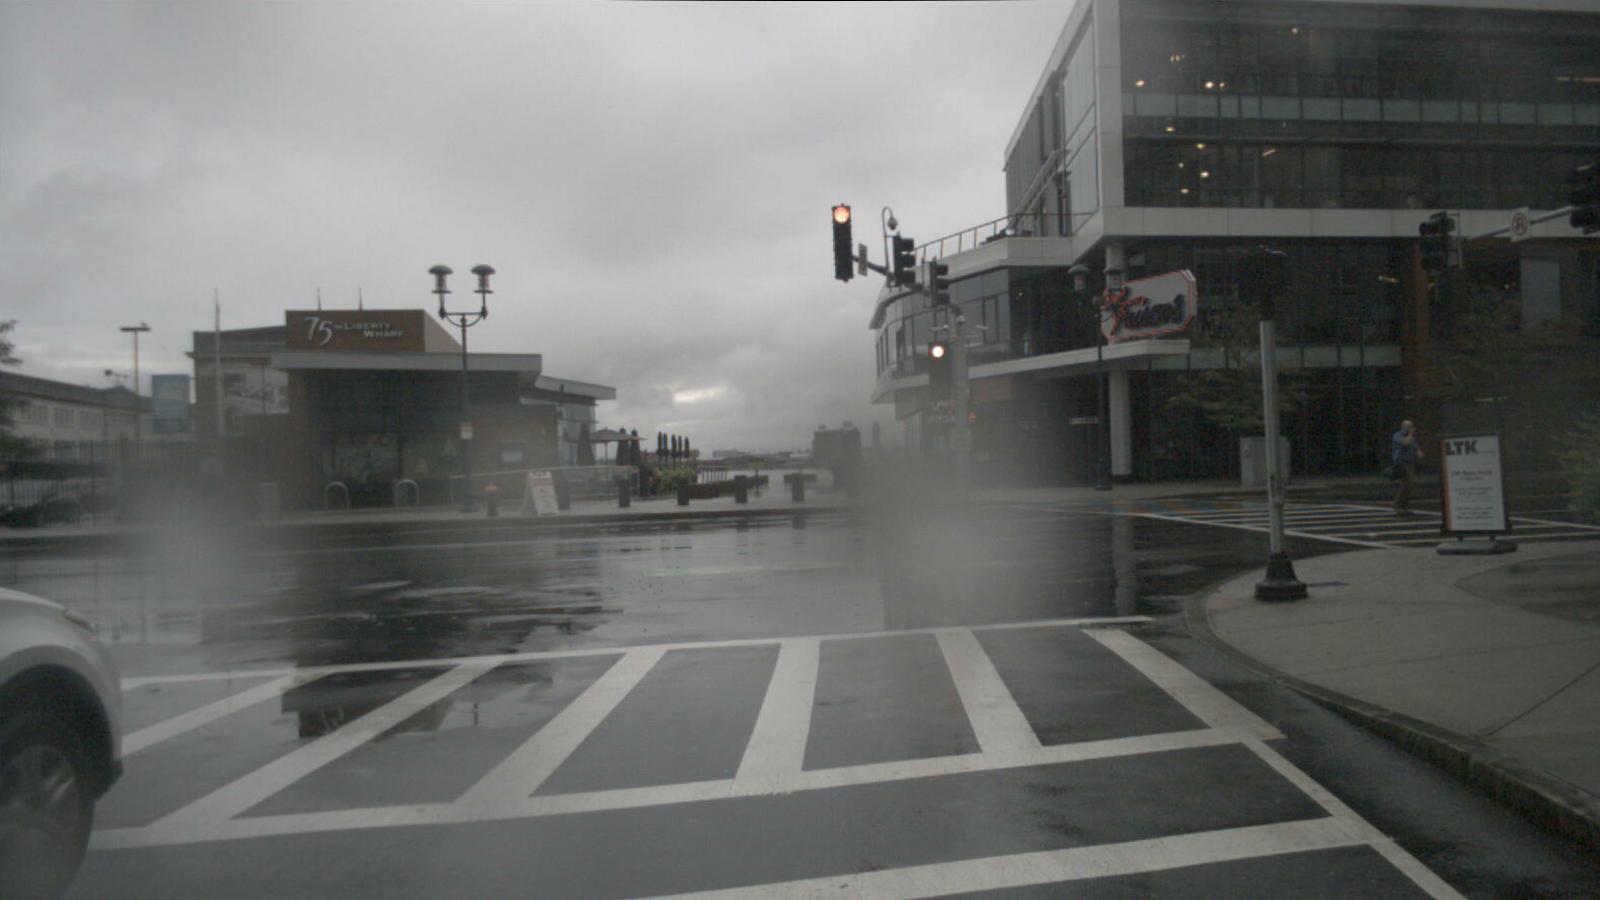
\includegraphics[width=6cm]{Figures/n008-2018-09-18-15-26-58-0400__CAM_FRONT__1537299148862404.jpg}\hypertarget{example1}\\
    {\tiny CAM\_FRONT}
}}
& \textbf{Q}: 
What is the target action of the ego vehicle? \\
& \textbf{GT Answer}: Stationary. \\
& \textbf{Q-only}: Go straight. \\
& \textbf{EM-VLM4AD}: Go straight. \\ 
& \textbf{Our}: Stationary. \\
\vspace{2em} & \vspace{2em} \\

\multirow{4}{*}{\parbox{6cm}{
    \centering
    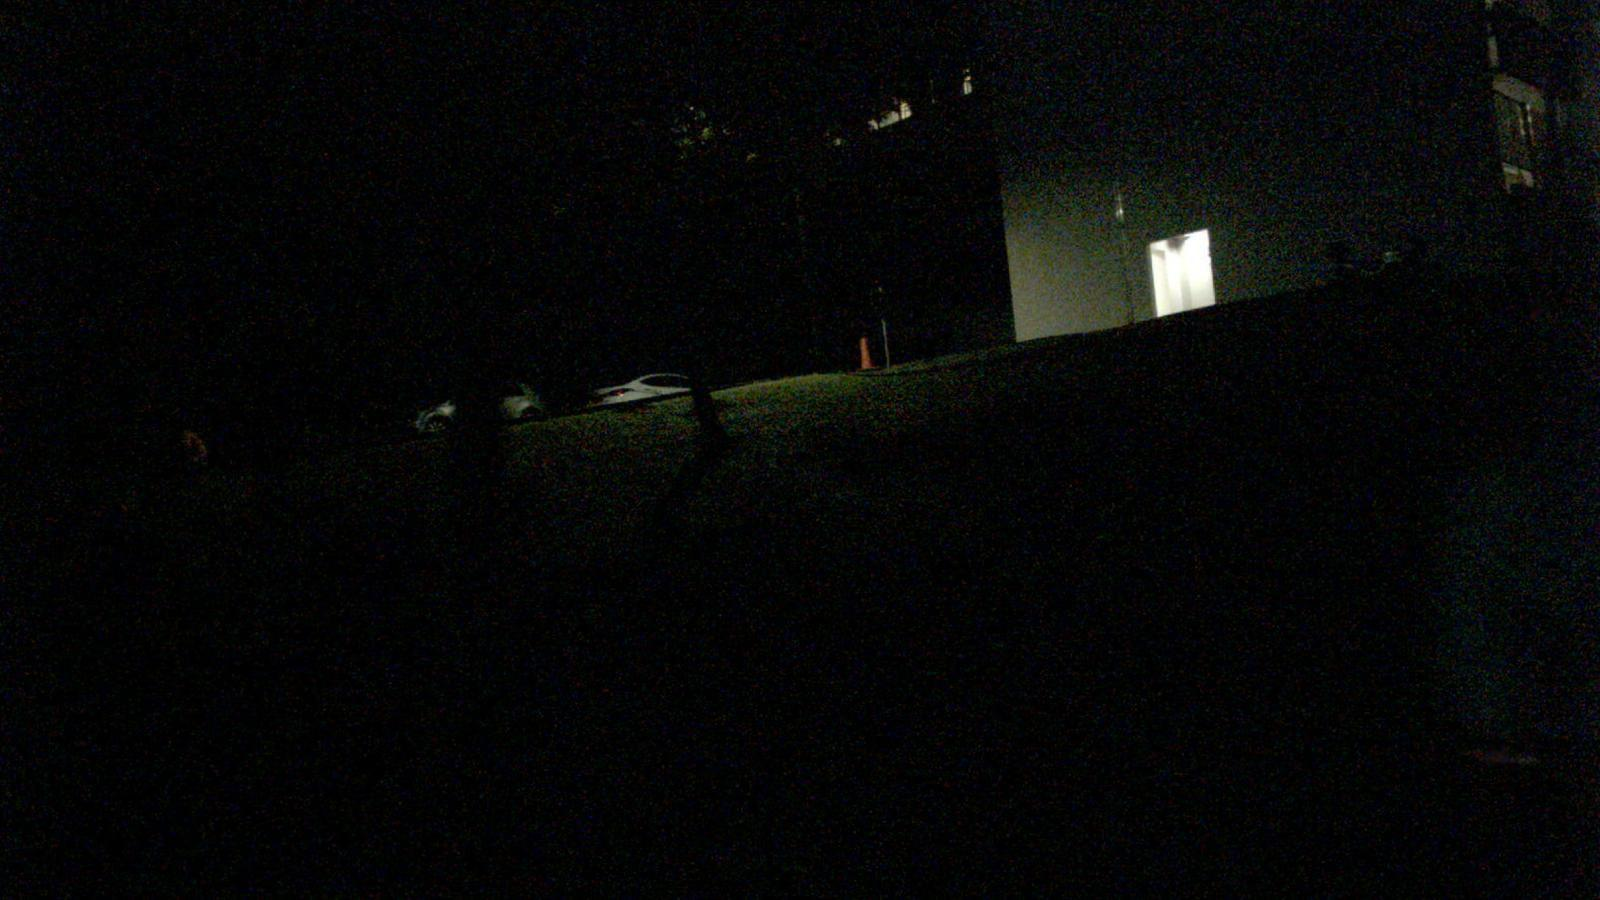
\includegraphics[width=6cm]{Figures/n015-2018-11-14-19-09-14+0800__CAM_BACK_LEFT__1542193883447423.jpg}\hypertarget{example2}\\
    {\tiny CAM\_BACK\_LEFT}
}}
& \textbf{Q}: What is the status of the pedestrian that is to the back left of the ego car? \\
& \textbf{GT Answer}: One pedestrian is standing. \\
& \textbf{Q-only}: The pedestrian to the back left of the ego car is moving. \\
& \textbf{EM-VLM4AD}: The pedestrian to the back left of the ego car is moving. \\ 
& \textbf{Our}: One pedestrian is standing. \\
\vspace{1em} & \vspace{1em} \\

\multirow{4}{*}{\parbox{6cm}{
    \centering
    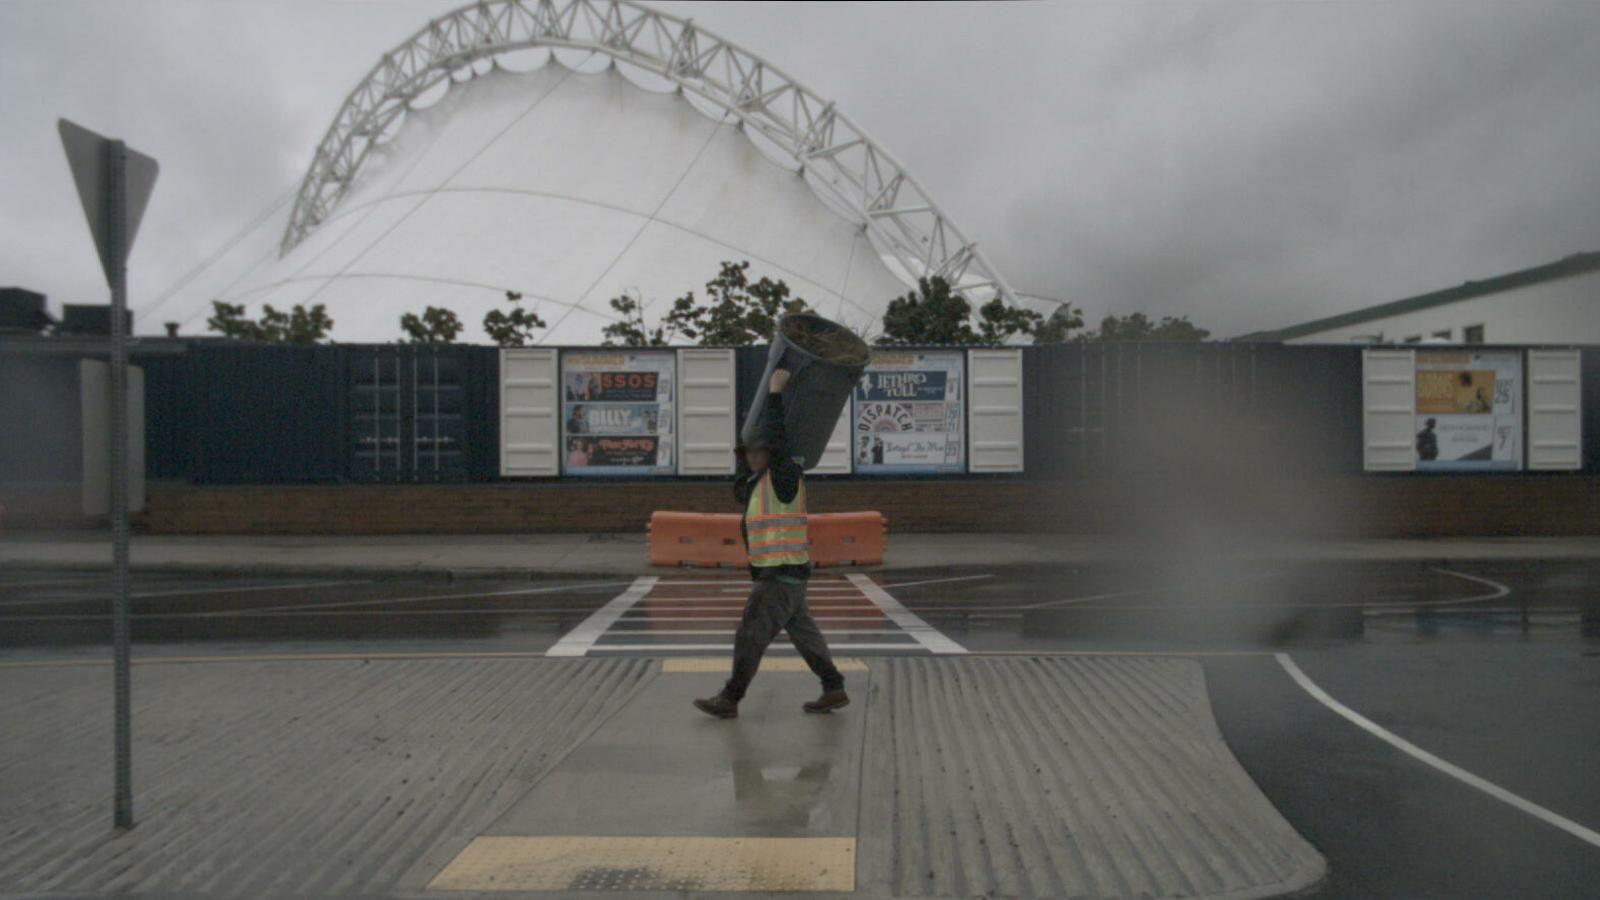
\includegraphics[width=6cm]{Figures/n008-2018-09-18-13-41-50-0400__CAM_BACK_LEFT__1537293297797405.jpg}\\
    {\tiny CAM\_BACK\_LEFT}
}}
& \textbf{Q}: What is the future state of \texttt{<c2,CAM\_BACK\_LEFT,805.0,512.5>}? \\
& \textbf{GT Answer}: Keep going straight. \\
& \textbf{Q-only}: Stationary. \\
& \textbf{EM-VLM4AD}: Stationary. \\ 
& \textbf{Our}: Keep going straight. \\
\vspace{2em} & \vspace{2em} \\

\multirow{4}{*}{\parbox{6cm}{
    \centering
    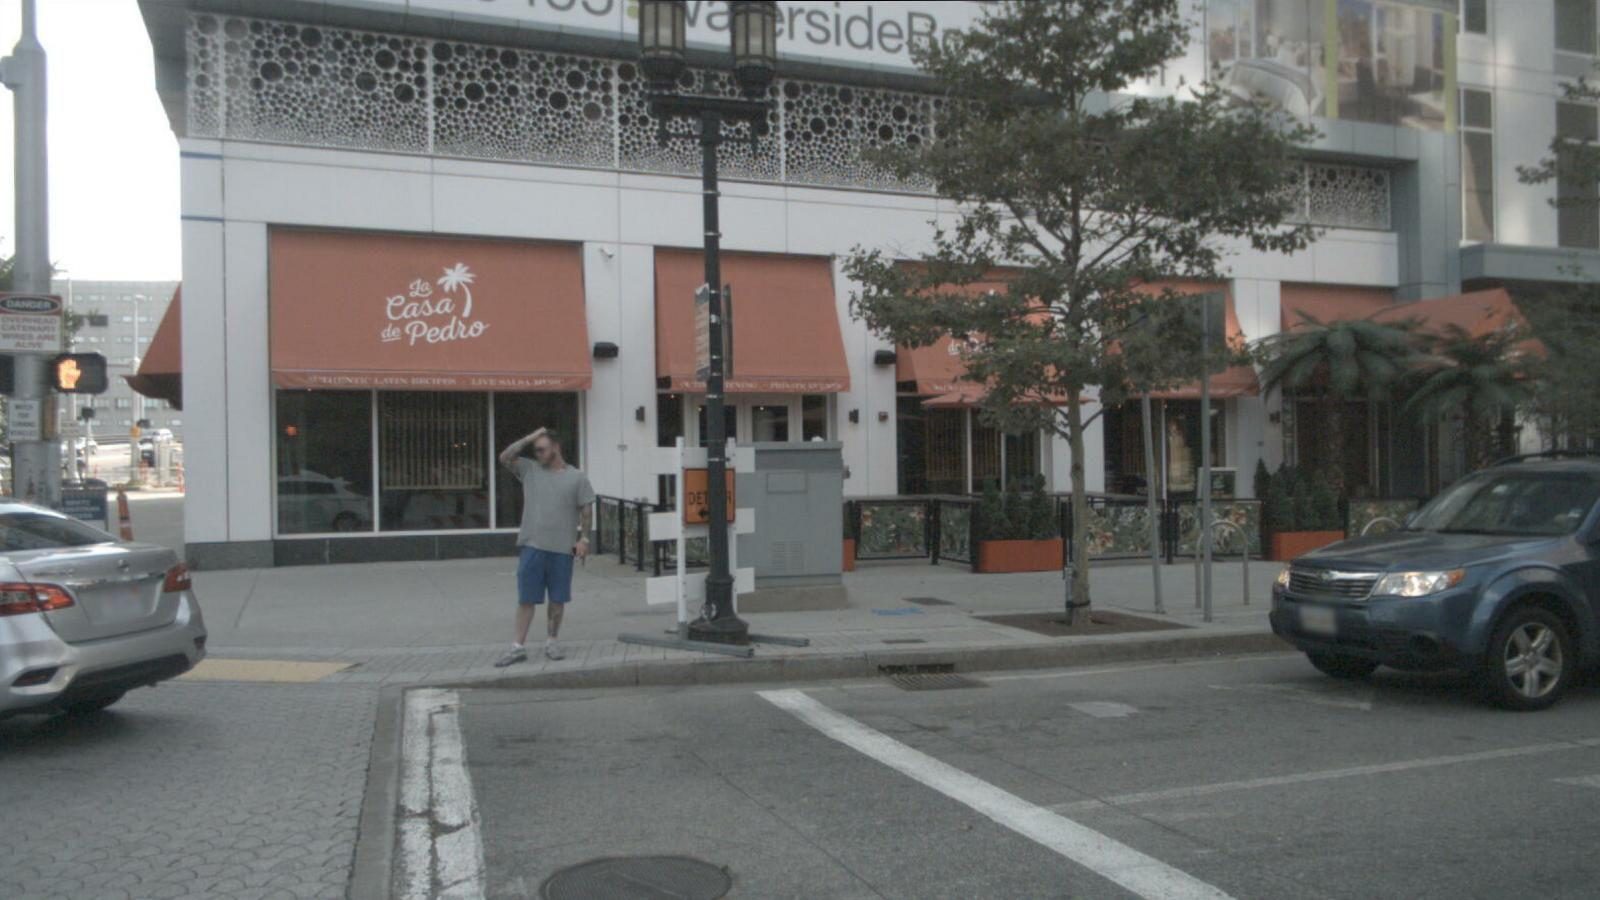
\includegraphics[width=6cm]{Figures/n008-2018-08-29-16-04-13-0400__CAM_BACK_RIGHT__1535573956528113.jpg}\\
    {\tiny CAM\_BACK\_RIGHT}
}}
& \textbf{Q}: What is the status of the car that is to the back right of the ego car? \\
& \textbf{GT Answer}: One car is moving. \\
& \textbf{Q-only}: One car is parked. \\
& \textbf{EM-VLM4AD}: One car is parked. \\ 
& \textbf{Our}: One car is moving. \\
\vspace{2em} & \vspace{2em} \\
\end{tabular}
    \caption{Cases Where Only Our Method Answered Correctly.}
    \label{tab:qualitative_examples_our}
\end{table}


However, these successes are likely coincidental, as we observed a similar number of cases where each individual method was the only one to answer correctly while the other two failed. And in most scenarios, all methods answered incorrectly. This suggests that no method consistently outperforms the others across all scenarios, despite our proposed method having a marginally higher metric score.


\begin{table}[htbp]
    \centering
\begin{tabular}{cp{9cm}}
\multirow{4}{*}{\parbox{6cm}{
    \centering
    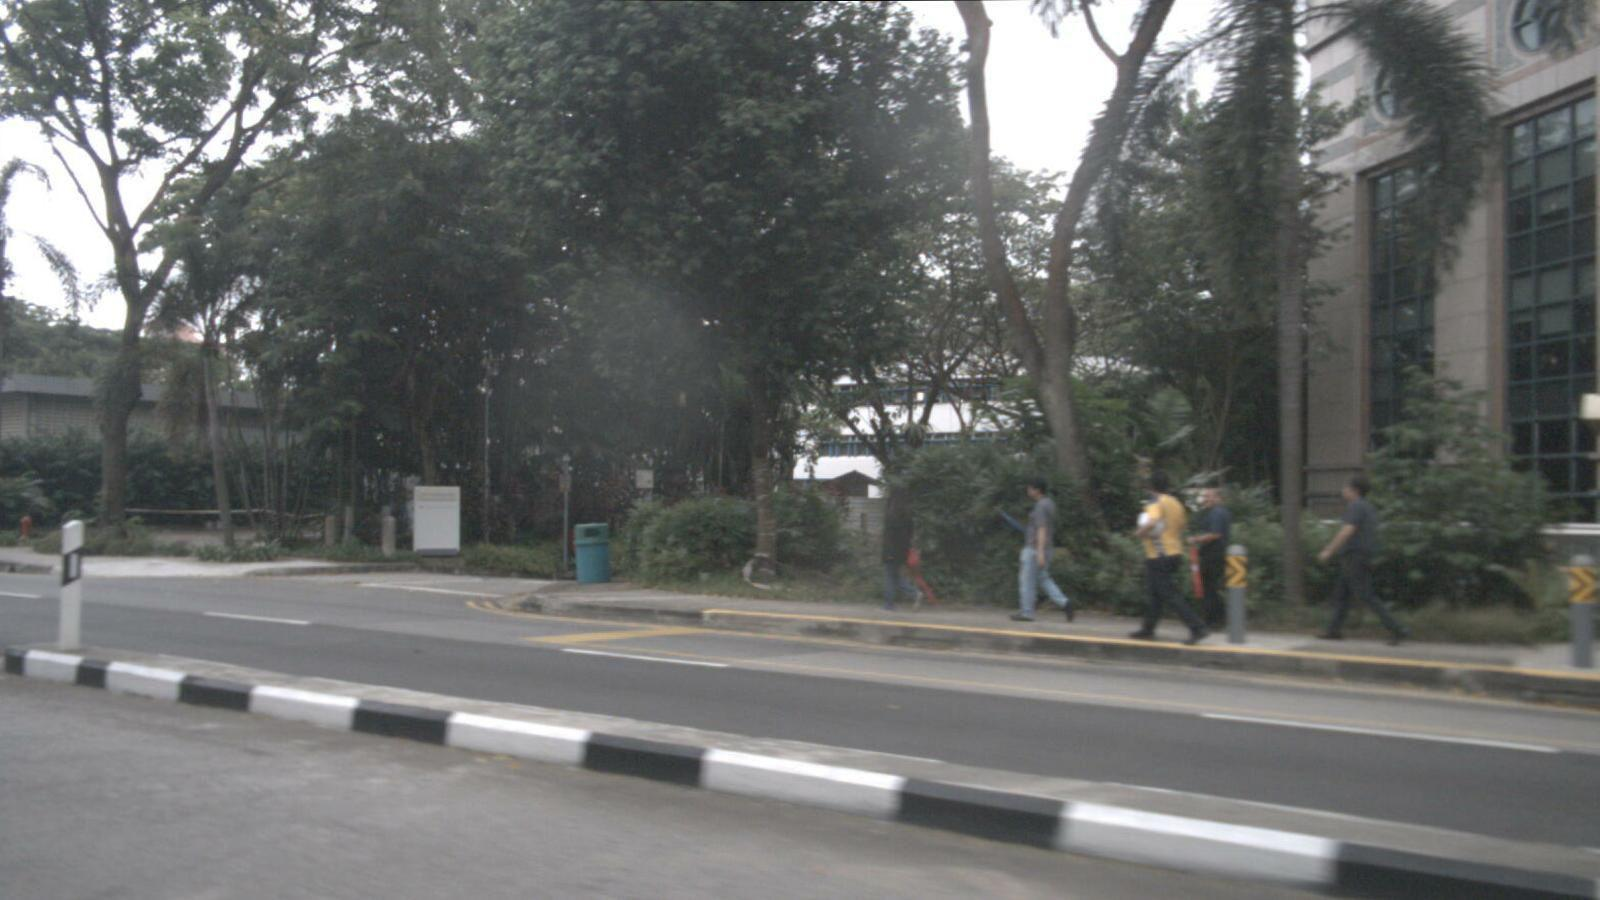
\includegraphics[width=6cm]{Figures/n015-2018-10-08-15-52-24+0800__CAM_FRONT_RIGHT__1538985706770339.jpg}\\
    {\tiny CAM\_FRONT\_RIGHT}
}}
& \textbf{Q}: What is the visual description of \texttt{<c1,CAM\_FRONT\_RIGHT,905.8,542.5>}? \\
& \textbf{GT Answer}: A woman wearing a black jacket. \\
& \textbf{Q-only}: White sedan. \\
& \textbf{EM-VLM4AD}: White van. \\ 
& \textbf{Our}: White sedan. \\
\vspace{2em} & \vspace{2em} \\

\multirow{4}{*}{\parbox{6cm}{
    \centering
    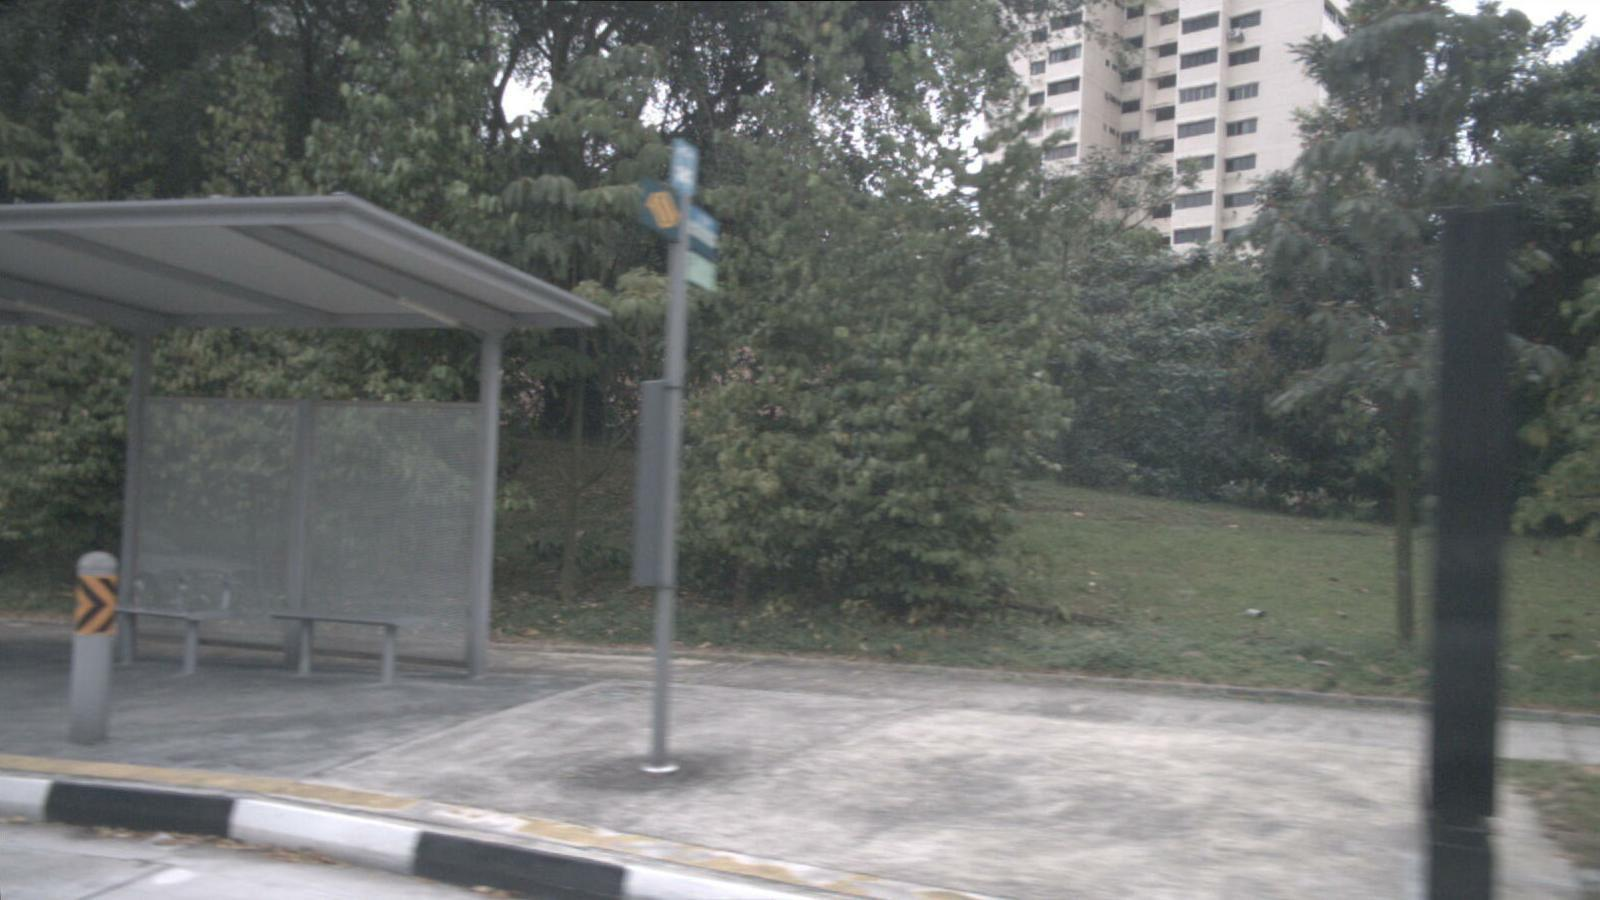
\includegraphics[width=6cm]{Figures/n015-2018-10-08-16-03-24+0800__CAM_BACK_LEFT__1538985816447423.jpg}\\
    {\tiny CAM\_BACK\_LEFT}
}}
& \textbf{Q}: Is \texttt{<c3,CAM\_BACK\_LEFT,91.8,645.9>} a traffic sign or a road barrier? \\
& \textbf{GT Answer}: Yes. \\
& \textbf{Q-only}: No. \\
& \textbf{EM-VLM4AD}: No. \\ 
& \textbf{Our}: No. \\
\vspace{2em} & \vspace{2em} \\
\end{tabular}
    \caption{Cases Where Every Method Failed.}
    \label{tab:qualitative_examples_all_fail}
\end{table}

\begin{table}[htbp]
    \centering
\begin{tabular}{cp{9cm}}
% \multirow{4}{*}{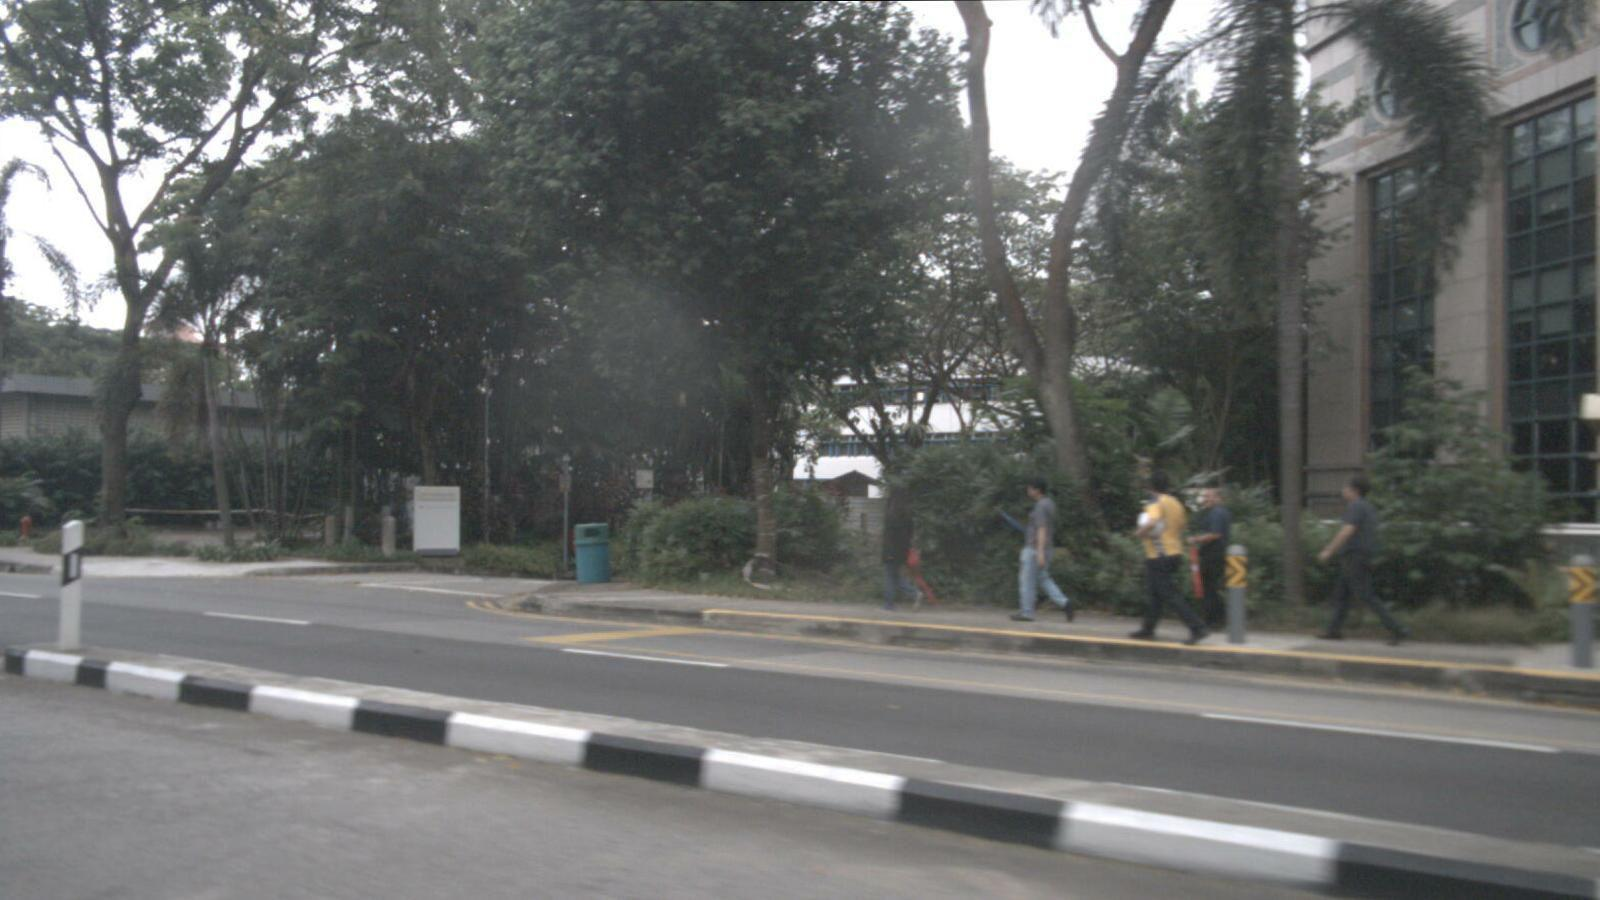
\includegraphics[width=5cm]{Figures/n015-2018-10-08-15-52-24+0800__CAM_FRONT_RIGHT__1538985706770339.jpg} } 

\multirow{4}{*}{\parbox{6cm}{
    \centering
    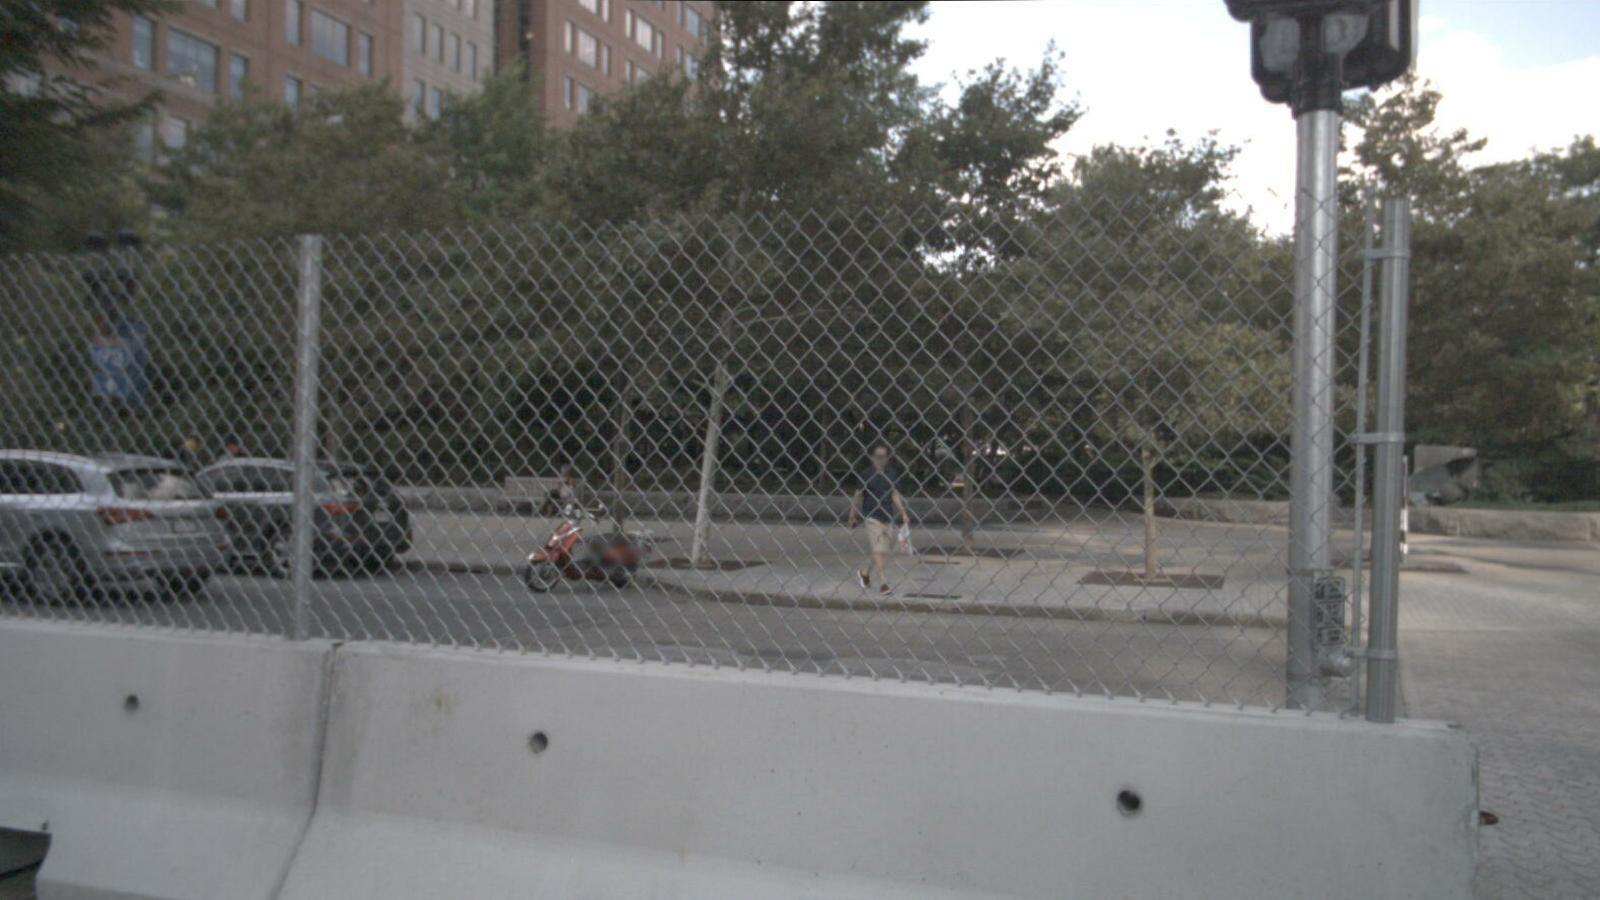
\includegraphics[width=6cm]{Figures/n008-2018-08-29-16-04-13-0400__CAM_BACK_LEFT__1535573956547405.jpg}\\
    {\tiny CAM\_BACK\_LEFT}
}}
& \textbf{Q}: Are there barriers to the back left of the ego car? \\
& \textbf{GT Answer}: Yes. \\
& \textbf{Q-only}: No. \\
& \textbf{EM-VLM4AD}: Yes. \\ 
& \textbf{Our}: No. \\
\vspace{3em} & \vspace{3em} \\

\multirow{4}{*}{\parbox{6cm}{
    \centering
    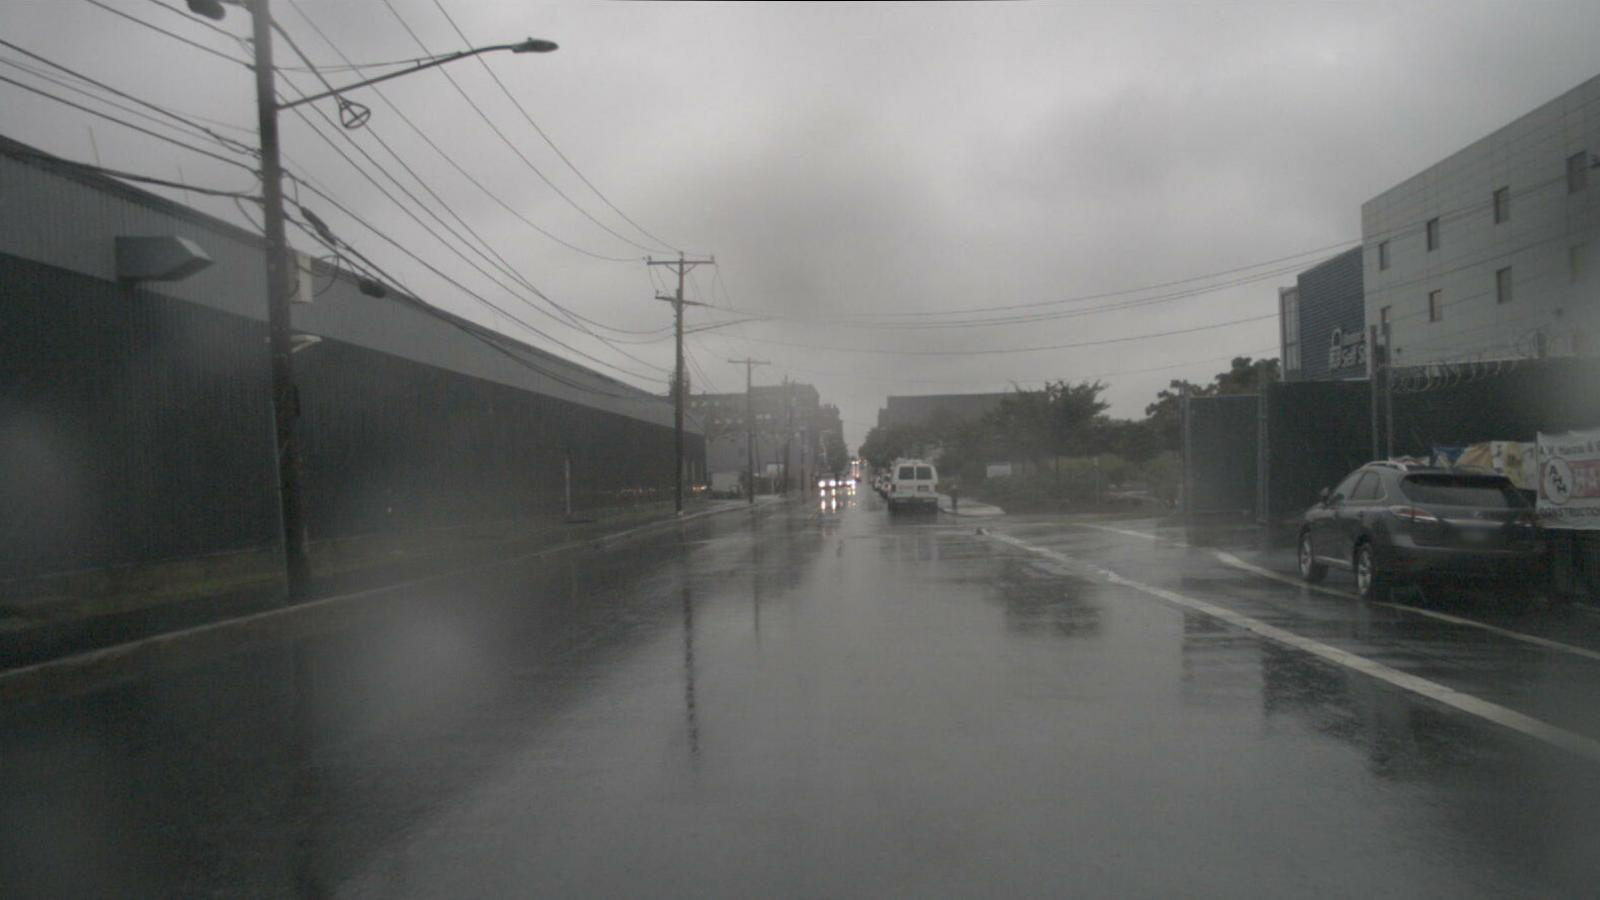
\includegraphics[width=6cm]{Figures/n008-2018-09-18-13-10-39-0400__CAM_FRONT__1537290748612404.jpg}\\
    {\tiny CAM\_FRONT}
}}
& \textbf{Q}: What is the visual description of \texttt{<c4,CAM\_FRONT,1428.3,524.2>}? \\
& \textbf{GT Answer}: Black SUV. \\
& \textbf{Q-only}: White sedan. \\
& \textbf{EM-VLM4AD}: Black SUV. \\ 
& \textbf{Our}: White sedan. \\
\vspace{2em} & \vspace{2em} \\
\end{tabular}
    \caption{Cases Where Every EM-VLM4AD Answered Correctly.}
    \label{tab:qualitative_examples_our}
\end{table}







\clearpage
% \section{\points{2} Future work and Limitations}
% Please thoroughly discuss the limitations of the proposed model. Where are all the places it does not work, phenomena it does not capture, places that ideally it can be improved. As guidance, there should be more things listed here than members of the team.
\section{Limitations}
\begin{enumerate}
\item \textbf{Trivial QA Pairs in DriveLM Dataset:}

Our ablation experiments revealed that our Q-only model, which predicts answers from questions without any camera or LiDAR input, performs surprisingly well.
The primary reason is the fact that the question-answer templates lack diversity and are often insufficiently challenging. In many cases, the answer can be inferred directly from the question without requiring visual or spatial reasoning. As a result, models may achieve high performance by simply learning the language priors and answer patterns, rather than leveraging multimodal visual inputs.
\begin{table}[htbp]
    \centering
    \begin{tabular}{|p{4.2cm}|p{2.3cm}|p{2.3cm}|p{2.5cm}|p{3.0cm}|}
        \hline
        \textbf{Question} & \textbf{GT Answer} & \textbf{Q-only} & \makecell{\textbf{EM-VLM4AD}\\(w/ cameras)} & \makecell{\textbf{Our}\\(w/ cameras \& lidar)} \\
        \hline
        % What actions taken by the ego vehicle can lead to a collision with \texttt{<c1,CAM\_FRONT\_LEFT>}? & Sharp left turn. & No such action will lead to a collision. & Sharp left turn. & Sharp left turn. \\
        % \hline
        What object would consider \texttt{<c3,CAM\_FRONT\_RIGHT,} \texttt{1010.7,411.4>} to be most relevant to its decision? & The ego vehicle. & The ego vehicle. & The ego vehicle. & The ego vehicle. \\
        \hline
        What actions taken by the ego vehicle can lead to a collision with \texttt{<c1,CAM\_FRONT\_RIGHT,} \texttt{215.8,664.2>}? & Sharp right turn. & Sharp right turn. & Sharp right turn. & Slight right turn. \\
        \hline
        % Is there any traffic element in the front view? & No, there are no traffic elements in the front view. & Yes, there are traffic elements in the front view. & Yes, there are traffic elements in the front view. & Yes, there are traffic elements in the front view. \\
        % \hline
        What is the moving status of object \texttt{<c1,CAM\_BACK,} \texttt{813.3,546.7>}? & Going ahead. & Going ahead. & Going ahead. & Going ahead. \\
        \hline
    \end{tabular}
    \caption{Trivially Correct Cases Caused by Poorly Constructed QA Pairs.}
    \label{tab:collision_responses}
\end{table}
    \item \textbf{Over-Reliance on Statistical Prior over Object Classes:}

    All models tend to ignore the visual input and instead rely on object frequency priors,  favoring common object classes irrespective of the actual scene.
\begin{table}[htbp]
    \centering
    \begin{tabular}{|p{4.2cm}|p{2.3cm}|p{2.3cm}|p{2.5cm}|p{3.0cm}|}
        \hline
        \textbf{Question} & \textbf{GT Answer} & \textbf{Q-only} & \makecell{\textbf{EM-VLM4AD}\\(w/ cameras)} & \makecell{\textbf{Our}\\(w/ cameras \& lidar)} \\
        \hline
        What is the visual description of \texttt{<c1,CAM\_FRONT\_RIGHT,} \texttt{905.8,542.5>}? & A woman wearing a black jacket. & White sedan. & White van. & White sedan. \\
        \hline
    \end{tabular}
    \caption{Models Favoring Frequent Object Classes over Visual Evidence.}
    \label{tab:collision_responses}
\end{table}
    \item \textbf{Lack of Explicit Spatial Grounding for Referenced Regions:}
    
    The visual features are fed into the language model as global embeddings of images (and lidar point clouds), without explicit mechanisms to retrieve the region of interest specified in the question (e.g., \texttt{<c3,CAM\_FRONT\_RIGHT,1010.7,411.4>}). This forces the language model to implicitly resolve spatial grounding from the global context, which is challenging given the lack of structured alignment between the referenced coordinates and the visual embeddings.
    \item \textbf{Poor Discriminative Power of Metrics:}
    
    The evaluation metrics we adopt (i.e., BLEU-4, ROUGE-L, and CIDEr) primarily emphasize exact n-gram or subsequence matches, often failing to capture deeper semantic equivalence between predicted and reference answers. While METEOR partially mitigates this issue through synonym matching and stemming, it still heavily relies on surface-level overlaps. Consequently, the discriminative power of these metrics remains limited, reducing the reliability of our experimental comparisons.
    
    %The metrics we use (i.e., BLEU-4, ROUGE-L, CIDEr) favor exact n-gram or subsequence matches, often overlooking semantic equivalence. METEOR partially addresses this by incorporating synonym matching and stemming, but still relies heavily on surface-level overlaps. This diminishes the discriminative power of our metrics, making our experiments less reliable.
\end{enumerate}

\section{Future Work}
Building on the identified limitations, we outline key challenges to address and potential directions for improvement:
\begin{enumerate}
    \item \textbf{Search for a High-Quality QA Dataset with Correct, Diverse, and Practical Questions:}

We have experimented with two driving scenario QA datasets. \textbf{NuScenes-QA} ~\cite{qian2024nuscenes} contains a substantial amount of misaligned QA pairs with incorrect answers and unnatural question phrasing. The current dataset, \textbf{DriveLM} ~\cite{gopalkrishnan2024multi}, provides generally correct answers but still lacks diversity, complexity, and practical relevance. To make any meaningful advances in the QA task will require identifying or constructing a higher-quality dataset with well-formed, non-trivial questions grounded in real-world driving scenarios.
    \item \textbf{Incorporating Temporal Context with Video Inputs:}

    The current setup answers questions based on single-frame camera and LiDAR inputs. This makes answering questions such as "Is the vehicle in front of me moving?" virtually impossible without relying on indirect visual cues (e.g., traffic lights). Incorporating video inputs would enable the model to capture temporal context directly and reason about dynamic scenes more effectively.
    \item \textbf{Simultaneous Map Reconstruction with SLAM Methods:}

    To generate informed answers in driving scenarios requires accurate geometric and visual grounding. Recent advances in SLAM methods, such as DUSt3R~\cite{wang2024dust3rgeometric3dvision}, enable real-time reconstruction of high-fidelity maps with precise geometry and visual appearance. Integrating such maps could significantly improve the quality of visual features and enhance the model's ability to answer spatially grounded QA tasks.
\end{enumerate}


\section{\points{1} Ethical Concerns and Considerations (unintentional, malicious, and dual-use)}

Our work on multimodal question answering (QA) in autonomous driving scenarios introduces several ethical considerations that must be addressed to ensure responsible deployment and development.

\subsection*{Unintentional Harm}

Despite efforts to improve model accuracy, several limitations—such as dataset misalignments, over-reliance on statistical priors, and lack of temporal context—can lead to \textbf{incorrect or misleading answers}. In safety-critical domains like autonomous driving, these inaccuracies could result in poor system decisions or misinterpretations during system evaluation. For instance, misidentifying whether a pedestrian is present or if a vehicle is moving could negatively impact driving policies, either during simulation or in downstream planning modules.

\subsection*{Malicious Use}

The models developed could be \textbf{misused to manipulate or deceive autonomous systems}. For example, adversarial actors could craft specific questions or manipulate sensor inputs to elicit false responses from the QA system, potentially influencing the decision-making of autonomous vehicles. Additionally, QA systems trained on scene understanding could be repurposed to \textbf{infer sensitive details} about environments or individuals, especially when deployed in non-consensual settings such as unauthorized surveillance.

\subsection*{Dual-Use Concerns}

While our system is designed to improve \textbf{driving safety} and \textbf{scene understanding}, the underlying technologies (e.g., multimodal perception, scene graph extraction, QA models) have \textbf{dual-use potential}. These methods could be adapted for military or law enforcement purposes, such as \textbf{surveillance systems} that analyze vehicular or pedestrian behavior at scale. This raises concerns about \textbf{privacy violations}, \textbf{mass surveillance}, or deployment in contexts lacking proper oversight.

\subsection*{Mitigation Strategies}

To address these concerns, we propose several mitigation strategies:

\begin{itemize}
    \item \textbf{Dataset auditing}: Ensure that datasets used for training and evaluation are well-aligned, diverse, and representative of real-world scenarios, minimizing biases and reducing the risk of unintended errors.
    \item \textbf{Robustness testing}: Incorporate adversarial testing frameworks to evaluate the model's resilience against manipulated inputs or misleading questions.
    \item \textbf{Transparency and explainability}: Develop mechanisms to provide \textbf{interpretable outputs} or rationales for model predictions, aiding human oversight and fostering trust.
    \item \textbf{Usage guidelines}: Define clear \textbf{ethical guidelines and usage policies} for deployment contexts, discouraging applications in scenarios that could violate privacy, safety, or human rights.
\end{itemize}

Addressing these ethical challenges is crucial for ensuring that the benefits of multimodal QA systems in autonomous driving are realized without causing harm or enabling misuse.

\newpage

\bibliography{references}
\bibliographystyle{iclr2024_conference}

%\appendix
%\section{Appendix}
%You may include other additional sections here.

\end{document}